% **************************************************************************************************************
% A Classic Thesis Style
% An Homage to The Elements of Typographic Style
%
% Copyright (C) 2012 Andr\'e Miede http://www.miede.de
%
% If you like the style then I would appreciate a postcard. My address
% can be found in the file ClassicThesis.pdf. A collection of the
% postcards I received so far is available online at
% http://postcards.miede.de
%
% License:
% This program is free software; you can redistribute it and/or modify
% it under the terms of the GNU General Public License as published by
% the Free Software Foundation; either version 2 of the License, or
% (at your option) any later version.
%
% This program is distributed in the hope that it will be useful,
% but WITHOUT ANY WARRANTY; without even the implied warranty of
% MERCHANTABILITY or FITNESS FOR A PARTICULAR PURPOSE. See the
% GNU General Public License for more details.
%
% You should have received a copy of the GNU General Public License
% along with this program; see the file COPYING. If not, write to
% the Free Software Foundation, Inc., 59 Temple Place - Suite 330,
% Boston, MA 02111-1307, USA.
%
% **************************************************************************************************************
% Note:
%    * You must not use "u etc. in strings/commands that will be spaced out (use \"u or real umlauts instead)
%    * New enumeration (small caps): \begin{aenumerate} \end{aenumerate}
%    * For margin notes: \marginpar or \graffito{}
%    * Do not use bold fonts in this style, it is designed around them
%    * Use tables as in the examples
%    * See classicthesis-config.tex for useful commands
% **************************************************************************************************************
% To Do:
%    * [high] Check this out: http://www.golatex.de/koma-script-warnung-in-verbindung-mit-listings-package-t2058.html
%    * [medium] mathbb in section-titles/chapter-titles => disappears somehow in headlines!!!
% **************************************************************************************************************
\RequirePackage{fix-cm} % fix some latex issues see: http://tug.org/texmf-dist/doc/latex/base/fixltx2e.pdf
\documentclass[%
    twoside,openright,titlepage,numbers=noenddot,headinclude,%1headlines,% letterpaper a4paper
    footinclude=true,cleardoublepage=empty,abstractoff, % <--- obsolete, remove (todo)
    BCOR=5mm,paper=a4,fontsize=11pt,%11pt,a4paper,%
    ngerman,american,%
    ]{scrreprt}

%********************************************************************
% Note: Make all your adjustments in here
%*******************************************************
% ****************************************************************************************************
% classicthesis-config.tex
% formerly known as loadpackages.sty, classicthesis-ldpkg.sty, and classicthesis-preamble.sty
% Use it at the beginning of your ClassicThesis.tex, or as a LaTeX Preamble
% in your ClassicThesis.{tex,lyx} with % ****************************************************************************************************
% classicthesis-config.tex
% formerly known as loadpackages.sty, classicthesis-ldpkg.sty, and classicthesis-preamble.sty
% Use it at the beginning of your ClassicThesis.tex, or as a LaTeX Preamble
% in your ClassicThesis.{tex,lyx} with % ****************************************************************************************************
% classicthesis-config.tex
% formerly known as loadpackages.sty, classicthesis-ldpkg.sty, and classicthesis-preamble.sty
% Use it at the beginning of your ClassicThesis.tex, or as a LaTeX Preamble
% in your ClassicThesis.{tex,lyx} with \input{classicthesis-config}
% ****************************************************************************************************
% If you like the classicthesis, then I would appreciate a postcard.
% My address can be found in the file ClassicThesis.pdf. A collection
% of the postcards I received so far is available online at
% http://postcards.miede.de
% ****************************************************************************************************


% ****************************************************************************************************
% 0. Set the encoding of your files. UTF-8 is the only sensible encoding nowadays. If you can't read
% äöüßáéçèê∂åëæƒÏ€ then change the encoding setting in your editor, not the line below. If your editor
% does not support utf8 use another editor!
% ****************************************************************************************************
\PassOptionsToPackage{utf8}{inputenc}
    \usepackage{inputenc}
\usepackage[OT4]{polski}

% ****************************************************************************************************
% 1. Configure classicthesis for your needs here, e.g., remove "drafting" below
% in order to deactivate the time-stamp on the pages
% ****************************************************************************************************
\PassOptionsToPackage{%
    eulerchapternumbers,listings,drafting,%
    pdfspacing,%floatperchapter,%linedheaders,%
    subfig,beramono,eulermath,parts%
}{classicthesis}
% ********************************************************************
% Available options for classicthesis.sty
% (see ClassicThesis.pdf for more information):
% drafting
% parts nochapters linedheaders
% eulerchapternumbers beramono eulermath pdfspacing minionprospacing
% tocaligned dottedtoc manychapters
% listings floatperchapter subfig
% ********************************************************************

% ********************************************************************
% Triggers for this config
% ********************************************************************
\usepackage{ifthen}
\newboolean{enable-backrefs} % enable backrefs in the bibliography
\setboolean{enable-backrefs}{false} % true false
% ****************************************************************************************************


% ****************************************************************************************************
% 2. Personal data and user ad-hoc commands
% ****************************************************************************************************
\newcommand{\myTitle}{A Classic Thesis Style\xspace}
\newcommand{\mySubtitle}{An Homage to The Elements of Typographic Style\xspace}
\newcommand{\myDegree}{Doktor-Ingenieur (Dr.-Ing.)\xspace}
\newcommand{\myName}{Andr\'e Miede\xspace}
\newcommand{\myProf}{Put name here\xspace}
\newcommand{\myOtherProf}{Put name here\xspace}
\newcommand{\mySupervisor}{Put name here\xspace}
\newcommand{\myFaculty}{Put data here\xspace}
\newcommand{\myDepartment}{Put data here\xspace}
\newcommand{\myUni}{Put data here\xspace}
\newcommand{\myLocation}{Darmstadt\xspace}
\newcommand{\myTime}{April 2013\xspace}
\newcommand{\myVersion}{version 4.1.1\xspace}

% ********************************************************************
% Setup, finetuning, and useful commands
% ********************************************************************
\newcounter{dummy} % necessary for correct hyperlinks (to index, bib, etc.)
\newlength{\abcd} % for ab..z string length calculation
\providecommand{\mLyX}{L\kern-.1667em\lower.25em\hbox{Y}\kern-.125emX\@}
\newcommand{\ie}{i.\,e.}
\newcommand{\Ie}{I.\,e.}
\newcommand{\eg}{e.\,g.}
\newcommand{\Eg}{E.\,g.}
% ****************************************************************************************************


% ****************************************************************************************************
% 3. Loading some handy packages
% ****************************************************************************************************
% ********************************************************************
% Packages with options that might require adjustments
% ********************************************************************
%\PassOptionsToPackage{ngerman,american}{babel} % change this to your language(s), main language last
% Spanish languages need extra options in order to work with this template
\PassOptionsToPackage{english,polish}{babel}
    \usepackage{babel}

\PassOptionsToPackage{square,numbers}{natbib}
    \usepackage{natbib}

\PassOptionsToPackage{fleqn}{amsmath} % math environments and more by the AMS
    \usepackage{amsmath}

% ********************************************************************
% General useful packages
% ********************************************************************
\PassOptionsToPackage{T1}{fontenc} % T2A for cyrillics
    \usepackage{fontenc}
\usepackage{textcomp} % fix warning with missing font shapes
\usepackage{fixltx2e} % fixes some LaTeX issues: http://tug.org/texmf-dist/doc/latex/base/fixltx2e.pdf
\usepackage{scrhack} % fix warnings when using KOMA with listings package
\usepackage{xspace} % to get the spacing after macros right
\usepackage{mparhack} % get marginpar right
\usepackage{algorithm}
\usepackage{algorithmic}
\floatname{algorithm}{Algorytm}
\renewcommand{\listalgorithmname}{Spis algorytmów}
\renewcommand{\algorithmicrequire}{\textbf{Asercje początkowe:}}
\usepackage{listings}
\usepackage{multicol}
\usepackage{moreverb}
\let\verbatiminput=\verbatimtabinput
\def\verbatimtabsize{4\relax}
\usepackage{makeidx}
\let\orgtheindex\theindex
\let\orgendtheindex\endtheindex
\def\theindex{%
\def\twocolumn{\begin{multicols}{2}}%
\def\onecolumn{}%
\clearpage
\orgtheindex
}
\def\endtheindex{%
\end{multicols}%
\orgendtheindex
}
\PassOptionsToPackage{printonlyused,smaller}{acronym}
    \usepackage{acronym} % nice macros for handling all acronyms in the thesis
%\renewcommand*{\acsfont}[1]{\textssc{#1}} % for MinionPro
\renewcommand{\bflabel}[1]{{#1}\hfill} % fix the list of acronyms
% ****************************************************************************************************


% ****************************************************************************************************
% 4. Setup floats: tables, (sub)figures, and captions
% ****************************************************************************************************
\usepackage{tabularx} % better tables
    \setlength{\extrarowheight}{3pt} % increase table row height
\newcommand{\tableheadline}[1]{\multicolumn{1}{c}{\spacedlowsmallcaps{#1}}}
\newcommand{\myfloatalign}{\centering} % to be used with each float for alignment
\usepackage{caption}
\captionsetup{format=hang,font=small}
\usepackage{subfig}
% ****************************************************************************************************


% ****************************************************************************************************
% 5. Setup code listings
% ****************************************************************************************************
\usepackage{listings}
%\lstset{emph={trueIndex,root},emphstyle=\color{BlueViolet}}%\underbar} % for special keywords
\lstset{%
    language=[LaTeX]Tex,%C++,
    keywordstyle=\color{RoyalBlue},%\bfseries,
    basicstyle=\small\ttfamily,
    %identifierstyle=\color{NavyBlue},
    commentstyle=\color{Green}\ttfamily,
    stringstyle=\rmfamily,
    numbers=none,%left,%
    numberstyle=\scriptsize,%\tiny
    stepnumber=5,
    numbersep=8pt,
    showstringspaces=false,
    breaklines=true,
    frameround=ftff,
    frame=single,
    belowcaptionskip=.75\baselineskip
    %frame=L
}
% ****************************************************************************************************


% ****************************************************************************************************
% 6. PDFLaTeX, hyperreferences and citation backreferences
% ****************************************************************************************************
% ********************************************************************
% Using PDFLaTeX
% ********************************************************************
\PassOptionsToPackage{pdftex,hyperfootnotes=false,pdfpagelabels}{hyperref}
    \usepackage{hyperref} % backref linktocpage pagebackref
\pdfcompresslevel=9
\pdfadjustspacing=1
\PassOptionsToPackage{pdftex}{graphicx}
    \usepackage{graphicx}

% ********************************************************************
% Setup the style of the backrefs from the bibliography
% (translate the options to any language you use)
% ********************************************************************
\newcommand{\backrefnotcitedstring}{\relax}%(Not cited.)
\newcommand{\backrefcitedsinglestring}[1]{(Cited on page~#1.)}
\newcommand{\backrefcitedmultistring}[1]{(Cited on pages~#1.)}
\ifthenelse{\boolean{enable-backrefs}}%
{%
    \PassOptionsToPackage{hyperpageref}{backref}
    \usepackage{backref} % to be loaded after hyperref package
    \renewcommand{\backreftwosep}{ and~} % separate 2 pages
    \renewcommand{\backreflastsep}{, and~} % separate last of longer list
    \renewcommand*{\backref}[1]{} % disable standard
    \renewcommand*{\backrefalt}[4]{% detailed backref
    \ifcase #1 %
        \backrefnotcitedstring%
    \or%
        \backrefcitedsinglestring{#2}%
    \else%
        \backrefcitedmultistring{#2}%
    \fi}%
}{\relax}

% ********************************************************************
% Hyperreferences
% ********************************************************************
\hypersetup{%
    %draft, % = no hyperlinking at all (useful in b/w printouts)
    colorlinks=true, linktocpage=true, pdfstartpage=3, pdfstartview=FitV,%
    % uncomment the following line if you want to have black links (e.g., for printing)
    %colorlinks=false, linktocpage=false, pdfborder={0 0 0}, pdfstartpage=3, pdfstartview=FitV,%
    breaklinks=true, pdfpagemode=UseNone, pageanchor=true, pdfpagemode=UseOutlines,%
    plainpages=false, bookmarksnumbered, bookmarksopen=true, bookmarksopenlevel=1,%
    hypertexnames=true, pdfhighlight=/O,%nesting=true,%frenchlinks,%
    urlcolor=webbrown, linkcolor=RoyalBlue, citecolor=webgreen, %pagecolor=RoyalBlue,%
    %urlcolor=Black, linkcolor=Black, citecolor=Black, %pagecolor=Black,%
    pdftitle={\myTitle},%
    pdfauthor={\textcopyright\ \myName, \myUni, \myFaculty},%
    pdfsubject={},%
    pdfkeywords={},%
    pdfcreator={pdfLaTeX},%
    pdfproducer={LaTeX with hyperref and classicthesis}%
}

% ********************************************************************
% Setup autoreferences
% ********************************************************************
% There are some issues regarding autorefnames
% http://www.ureader.de/msg/136221647.aspx
% http://www.tex.ac.uk/cgi-bin/texfaq2html?label=latexwords
% you have to redefine the makros for the
% language you use, e.g., american, ngerman
% (as chosen when loading babel/AtBeginDocument)
% ********************************************************************
\makeatletter
\@ifpackageloaded{babel}%
    {%
        \addto\extrasamerican{%
            \renewcommand*{\figureautorefname}{Figure}%
            \renewcommand*{\tableautorefname}{Table}%
            \renewcommand*{\partautorefname}{Part}%
            \renewcommand*{\chapterautorefname}{Chapter}%
            \renewcommand*{\sectionautorefname}{Section}%
            \renewcommand*{\subsectionautorefname}{Section}%
            \renewcommand*{\subsubsectionautorefname}{Section}%
        }%
        \addto\extrasngerman{%
            \renewcommand*{\paragraphautorefname}{Absatz}%
            \renewcommand*{\subparagraphautorefname}{Unterabsatz}%
            \renewcommand*{\footnoteautorefname}{Fu\"snote}%
            \renewcommand*{\FancyVerbLineautorefname}{Zeile}%
            \renewcommand*{\theoremautorefname}{Theorem}%
            \renewcommand*{\appendixautorefname}{Anhang}%
            \renewcommand*{\equationautorefname}{Gleichung}%
            \renewcommand*{\itemautorefname}{Punkt}%
        }%
        % Fix to getting autorefs for subfigures right (thanks to Belinda Vogt for changing the definition)
        \providecommand{\subfigureautorefname}{\figureautorefname}%
    }{\relax}
\makeatother


% ****************************************************************************************************
% 7. Last calls before the bar closes
% ****************************************************************************************************
% ********************************************************************
% Development Stuff
% ********************************************************************
\listfiles
%\PassOptionsToPackage{l2tabu,orthodox,abort}{nag}
%    \usepackage{nag}
%\PassOptionsToPackage{warning, all}{onlyamsmath}
%    \usepackage{onlyamsmath}

% ********************************************************************
% Last, but not least...
% ********************************************************************
\usepackage{classicthesis}
% ****************************************************************************************************


% ****************************************************************************************************
% 8. Further adjustments (experimental)
% ****************************************************************************************************
% ********************************************************************
% Changing the text area
% ********************************************************************
%\linespread{1.05} % a bit more for Palatino
%\areaset[current]{312pt}{761pt} % 686 (factor 2.2) + 33 head + 42 head \the\footskip
%\setlength{\marginparwidth}{7em}%
%\setlength{\marginparsep}{2em}%

% ********************************************************************
% Using different fonts
% ********************************************************************
%\usepackage[oldstylenums]{kpfonts} % oldstyle notextcomp
%\usepackage[osf]{libertine}
%\usepackage{hfoldsty} % Computer Modern with osf
%\usepackage[light,condensed,math]{iwona}
%\renewcommand{\sfdefault}{iwona}
%\usepackage{lmodern} % <-- no osf support :-(
%\usepackage[urw-garamond]{mathdesign} <-- no osf support :-(
% ****************************************************************************************************

% ****************************************************************************************************
% If you like the classicthesis, then I would appreciate a postcard.
% My address can be found in the file ClassicThesis.pdf. A collection
% of the postcards I received so far is available online at
% http://postcards.miede.de
% ****************************************************************************************************


% ****************************************************************************************************
% 0. Set the encoding of your files. UTF-8 is the only sensible encoding nowadays. If you can't read
% äöüßáéçèê∂åëæƒÏ€ then change the encoding setting in your editor, not the line below. If your editor
% does not support utf8 use another editor!
% ****************************************************************************************************
\PassOptionsToPackage{utf8}{inputenc}
    \usepackage{inputenc}
\usepackage[OT4]{polski}

% ****************************************************************************************************
% 1. Configure classicthesis for your needs here, e.g., remove "drafting" below
% in order to deactivate the time-stamp on the pages
% ****************************************************************************************************
\PassOptionsToPackage{%
    eulerchapternumbers,listings,drafting,%
    pdfspacing,%floatperchapter,%linedheaders,%
    subfig,beramono,eulermath,parts%
}{classicthesis}
% ********************************************************************
% Available options for classicthesis.sty
% (see ClassicThesis.pdf for more information):
% drafting
% parts nochapters linedheaders
% eulerchapternumbers beramono eulermath pdfspacing minionprospacing
% tocaligned dottedtoc manychapters
% listings floatperchapter subfig
% ********************************************************************

% ********************************************************************
% Triggers for this config
% ********************************************************************
\usepackage{ifthen}
\newboolean{enable-backrefs} % enable backrefs in the bibliography
\setboolean{enable-backrefs}{false} % true false
% ****************************************************************************************************


% ****************************************************************************************************
% 2. Personal data and user ad-hoc commands
% ****************************************************************************************************
\newcommand{\myTitle}{A Classic Thesis Style\xspace}
\newcommand{\mySubtitle}{An Homage to The Elements of Typographic Style\xspace}
\newcommand{\myDegree}{Doktor-Ingenieur (Dr.-Ing.)\xspace}
\newcommand{\myName}{Andr\'e Miede\xspace}
\newcommand{\myProf}{Put name here\xspace}
\newcommand{\myOtherProf}{Put name here\xspace}
\newcommand{\mySupervisor}{Put name here\xspace}
\newcommand{\myFaculty}{Put data here\xspace}
\newcommand{\myDepartment}{Put data here\xspace}
\newcommand{\myUni}{Put data here\xspace}
\newcommand{\myLocation}{Darmstadt\xspace}
\newcommand{\myTime}{April 2013\xspace}
\newcommand{\myVersion}{version 4.1.1\xspace}

% ********************************************************************
% Setup, finetuning, and useful commands
% ********************************************************************
\newcounter{dummy} % necessary for correct hyperlinks (to index, bib, etc.)
\newlength{\abcd} % for ab..z string length calculation
\providecommand{\mLyX}{L\kern-.1667em\lower.25em\hbox{Y}\kern-.125emX\@}
\newcommand{\ie}{i.\,e.}
\newcommand{\Ie}{I.\,e.}
\newcommand{\eg}{e.\,g.}
\newcommand{\Eg}{E.\,g.}
% ****************************************************************************************************


% ****************************************************************************************************
% 3. Loading some handy packages
% ****************************************************************************************************
% ********************************************************************
% Packages with options that might require adjustments
% ********************************************************************
%\PassOptionsToPackage{ngerman,american}{babel} % change this to your language(s), main language last
% Spanish languages need extra options in order to work with this template
\PassOptionsToPackage{english,polish}{babel}
    \usepackage{babel}

\PassOptionsToPackage{square,numbers}{natbib}
    \usepackage{natbib}

\PassOptionsToPackage{fleqn}{amsmath} % math environments and more by the AMS
    \usepackage{amsmath}

% ********************************************************************
% General useful packages
% ********************************************************************
\PassOptionsToPackage{T1}{fontenc} % T2A for cyrillics
    \usepackage{fontenc}
\usepackage{textcomp} % fix warning with missing font shapes
\usepackage{fixltx2e} % fixes some LaTeX issues: http://tug.org/texmf-dist/doc/latex/base/fixltx2e.pdf
\usepackage{scrhack} % fix warnings when using KOMA with listings package
\usepackage{xspace} % to get the spacing after macros right
\usepackage{mparhack} % get marginpar right
\usepackage{algorithm}
\usepackage{algorithmic}
\floatname{algorithm}{Algorytm}
\renewcommand{\listalgorithmname}{Spis algorytmów}
\renewcommand{\algorithmicrequire}{\textbf{Asercje początkowe:}}
\usepackage{listings}
\usepackage{multicol}
\usepackage{moreverb}
\let\verbatiminput=\verbatimtabinput
\def\verbatimtabsize{4\relax}
\usepackage{makeidx}
\let\orgtheindex\theindex
\let\orgendtheindex\endtheindex
\def\theindex{%
\def\twocolumn{\begin{multicols}{2}}%
\def\onecolumn{}%
\clearpage
\orgtheindex
}
\def\endtheindex{%
\end{multicols}%
\orgendtheindex
}
\PassOptionsToPackage{printonlyused,smaller}{acronym}
    \usepackage{acronym} % nice macros for handling all acronyms in the thesis
%\renewcommand*{\acsfont}[1]{\textssc{#1}} % for MinionPro
\renewcommand{\bflabel}[1]{{#1}\hfill} % fix the list of acronyms
% ****************************************************************************************************


% ****************************************************************************************************
% 4. Setup floats: tables, (sub)figures, and captions
% ****************************************************************************************************
\usepackage{tabularx} % better tables
    \setlength{\extrarowheight}{3pt} % increase table row height
\newcommand{\tableheadline}[1]{\multicolumn{1}{c}{\spacedlowsmallcaps{#1}}}
\newcommand{\myfloatalign}{\centering} % to be used with each float for alignment
\usepackage{caption}
\captionsetup{format=hang,font=small}
\usepackage{subfig}
% ****************************************************************************************************


% ****************************************************************************************************
% 5. Setup code listings
% ****************************************************************************************************
\usepackage{listings}
%\lstset{emph={trueIndex,root},emphstyle=\color{BlueViolet}}%\underbar} % for special keywords
\lstset{%
    language=[LaTeX]Tex,%C++,
    keywordstyle=\color{RoyalBlue},%\bfseries,
    basicstyle=\small\ttfamily,
    %identifierstyle=\color{NavyBlue},
    commentstyle=\color{Green}\ttfamily,
    stringstyle=\rmfamily,
    numbers=none,%left,%
    numberstyle=\scriptsize,%\tiny
    stepnumber=5,
    numbersep=8pt,
    showstringspaces=false,
    breaklines=true,
    frameround=ftff,
    frame=single,
    belowcaptionskip=.75\baselineskip
    %frame=L
}
% ****************************************************************************************************


% ****************************************************************************************************
% 6. PDFLaTeX, hyperreferences and citation backreferences
% ****************************************************************************************************
% ********************************************************************
% Using PDFLaTeX
% ********************************************************************
\PassOptionsToPackage{pdftex,hyperfootnotes=false,pdfpagelabels}{hyperref}
    \usepackage{hyperref} % backref linktocpage pagebackref
\pdfcompresslevel=9
\pdfadjustspacing=1
\PassOptionsToPackage{pdftex}{graphicx}
    \usepackage{graphicx}

% ********************************************************************
% Setup the style of the backrefs from the bibliography
% (translate the options to any language you use)
% ********************************************************************
\newcommand{\backrefnotcitedstring}{\relax}%(Not cited.)
\newcommand{\backrefcitedsinglestring}[1]{(Cited on page~#1.)}
\newcommand{\backrefcitedmultistring}[1]{(Cited on pages~#1.)}
\ifthenelse{\boolean{enable-backrefs}}%
{%
    \PassOptionsToPackage{hyperpageref}{backref}
    \usepackage{backref} % to be loaded after hyperref package
    \renewcommand{\backreftwosep}{ and~} % separate 2 pages
    \renewcommand{\backreflastsep}{, and~} % separate last of longer list
    \renewcommand*{\backref}[1]{} % disable standard
    \renewcommand*{\backrefalt}[4]{% detailed backref
    \ifcase #1 %
        \backrefnotcitedstring%
    \or%
        \backrefcitedsinglestring{#2}%
    \else%
        \backrefcitedmultistring{#2}%
    \fi}%
}{\relax}

% ********************************************************************
% Hyperreferences
% ********************************************************************
\hypersetup{%
    %draft, % = no hyperlinking at all (useful in b/w printouts)
    colorlinks=true, linktocpage=true, pdfstartpage=3, pdfstartview=FitV,%
    % uncomment the following line if you want to have black links (e.g., for printing)
    %colorlinks=false, linktocpage=false, pdfborder={0 0 0}, pdfstartpage=3, pdfstartview=FitV,%
    breaklinks=true, pdfpagemode=UseNone, pageanchor=true, pdfpagemode=UseOutlines,%
    plainpages=false, bookmarksnumbered, bookmarksopen=true, bookmarksopenlevel=1,%
    hypertexnames=true, pdfhighlight=/O,%nesting=true,%frenchlinks,%
    urlcolor=webbrown, linkcolor=RoyalBlue, citecolor=webgreen, %pagecolor=RoyalBlue,%
    %urlcolor=Black, linkcolor=Black, citecolor=Black, %pagecolor=Black,%
    pdftitle={\myTitle},%
    pdfauthor={\textcopyright\ \myName, \myUni, \myFaculty},%
    pdfsubject={},%
    pdfkeywords={},%
    pdfcreator={pdfLaTeX},%
    pdfproducer={LaTeX with hyperref and classicthesis}%
}

% ********************************************************************
% Setup autoreferences
% ********************************************************************
% There are some issues regarding autorefnames
% http://www.ureader.de/msg/136221647.aspx
% http://www.tex.ac.uk/cgi-bin/texfaq2html?label=latexwords
% you have to redefine the makros for the
% language you use, e.g., american, ngerman
% (as chosen when loading babel/AtBeginDocument)
% ********************************************************************
\makeatletter
\@ifpackageloaded{babel}%
    {%
        \addto\extrasamerican{%
            \renewcommand*{\figureautorefname}{Figure}%
            \renewcommand*{\tableautorefname}{Table}%
            \renewcommand*{\partautorefname}{Part}%
            \renewcommand*{\chapterautorefname}{Chapter}%
            \renewcommand*{\sectionautorefname}{Section}%
            \renewcommand*{\subsectionautorefname}{Section}%
            \renewcommand*{\subsubsectionautorefname}{Section}%
        }%
        \addto\extrasngerman{%
            \renewcommand*{\paragraphautorefname}{Absatz}%
            \renewcommand*{\subparagraphautorefname}{Unterabsatz}%
            \renewcommand*{\footnoteautorefname}{Fu\"snote}%
            \renewcommand*{\FancyVerbLineautorefname}{Zeile}%
            \renewcommand*{\theoremautorefname}{Theorem}%
            \renewcommand*{\appendixautorefname}{Anhang}%
            \renewcommand*{\equationautorefname}{Gleichung}%
            \renewcommand*{\itemautorefname}{Punkt}%
        }%
        % Fix to getting autorefs for subfigures right (thanks to Belinda Vogt for changing the definition)
        \providecommand{\subfigureautorefname}{\figureautorefname}%
    }{\relax}
\makeatother


% ****************************************************************************************************
% 7. Last calls before the bar closes
% ****************************************************************************************************
% ********************************************************************
% Development Stuff
% ********************************************************************
\listfiles
%\PassOptionsToPackage{l2tabu,orthodox,abort}{nag}
%    \usepackage{nag}
%\PassOptionsToPackage{warning, all}{onlyamsmath}
%    \usepackage{onlyamsmath}

% ********************************************************************
% Last, but not least...
% ********************************************************************
\usepackage{classicthesis}
% ****************************************************************************************************


% ****************************************************************************************************
% 8. Further adjustments (experimental)
% ****************************************************************************************************
% ********************************************************************
% Changing the text area
% ********************************************************************
%\linespread{1.05} % a bit more for Palatino
%\areaset[current]{312pt}{761pt} % 686 (factor 2.2) + 33 head + 42 head \the\footskip
%\setlength{\marginparwidth}{7em}%
%\setlength{\marginparsep}{2em}%

% ********************************************************************
% Using different fonts
% ********************************************************************
%\usepackage[oldstylenums]{kpfonts} % oldstyle notextcomp
%\usepackage[osf]{libertine}
%\usepackage{hfoldsty} % Computer Modern with osf
%\usepackage[light,condensed,math]{iwona}
%\renewcommand{\sfdefault}{iwona}
%\usepackage{lmodern} % <-- no osf support :-(
%\usepackage[urw-garamond]{mathdesign} <-- no osf support :-(
% ****************************************************************************************************

% ****************************************************************************************************
% If you like the classicthesis, then I would appreciate a postcard.
% My address can be found in the file ClassicThesis.pdf. A collection
% of the postcards I received so far is available online at
% http://postcards.miede.de
% ****************************************************************************************************


% ****************************************************************************************************
% 0. Set the encoding of your files. UTF-8 is the only sensible encoding nowadays. If you can't read
% äöüßáéçèê∂åëæƒÏ€ then change the encoding setting in your editor, not the line below. If your editor
% does not support utf8 use another editor!
% ****************************************************************************************************
\PassOptionsToPackage{utf8}{inputenc}
    \usepackage{inputenc}
\usepackage[OT4]{polski}

% ****************************************************************************************************
% 1. Configure classicthesis for your needs here, e.g., remove "drafting" below
% in order to deactivate the time-stamp on the pages
% ****************************************************************************************************
\PassOptionsToPackage{%
    eulerchapternumbers,listings,drafting,%
    pdfspacing,%floatperchapter,%linedheaders,%
    subfig,beramono,eulermath,parts%
}{classicthesis}
% ********************************************************************
% Available options for classicthesis.sty
% (see ClassicThesis.pdf for more information):
% drafting
% parts nochapters linedheaders
% eulerchapternumbers beramono eulermath pdfspacing minionprospacing
% tocaligned dottedtoc manychapters
% listings floatperchapter subfig
% ********************************************************************

% ********************************************************************
% Triggers for this config
% ********************************************************************
\usepackage{ifthen}
\newboolean{enable-backrefs} % enable backrefs in the bibliography
\setboolean{enable-backrefs}{false} % true false
% ****************************************************************************************************


% ****************************************************************************************************
% 2. Personal data and user ad-hoc commands
% ****************************************************************************************************
\newcommand{\myTitle}{A Classic Thesis Style\xspace}
\newcommand{\mySubtitle}{An Homage to The Elements of Typographic Style\xspace}
\newcommand{\myDegree}{Doktor-Ingenieur (Dr.-Ing.)\xspace}
\newcommand{\myName}{Andr\'e Miede\xspace}
\newcommand{\myProf}{Put name here\xspace}
\newcommand{\myOtherProf}{Put name here\xspace}
\newcommand{\mySupervisor}{Put name here\xspace}
\newcommand{\myFaculty}{Put data here\xspace}
\newcommand{\myDepartment}{Put data here\xspace}
\newcommand{\myUni}{Put data here\xspace}
\newcommand{\myLocation}{Darmstadt\xspace}
\newcommand{\myTime}{April 2013\xspace}
\newcommand{\myVersion}{version 4.1.1\xspace}

% ********************************************************************
% Setup, finetuning, and useful commands
% ********************************************************************
\newcounter{dummy} % necessary for correct hyperlinks (to index, bib, etc.)
\newlength{\abcd} % for ab..z string length calculation
\providecommand{\mLyX}{L\kern-.1667em\lower.25em\hbox{Y}\kern-.125emX\@}
\newcommand{\ie}{i.\,e.}
\newcommand{\Ie}{I.\,e.}
\newcommand{\eg}{e.\,g.}
\newcommand{\Eg}{E.\,g.}
% ****************************************************************************************************


% ****************************************************************************************************
% 3. Loading some handy packages
% ****************************************************************************************************
% ********************************************************************
% Packages with options that might require adjustments
% ********************************************************************
%\PassOptionsToPackage{ngerman,american}{babel} % change this to your language(s), main language last
% Spanish languages need extra options in order to work with this template
\PassOptionsToPackage{english,polish}{babel}
    \usepackage{babel}

\PassOptionsToPackage{square,numbers}{natbib}
    \usepackage{natbib}

\PassOptionsToPackage{fleqn}{amsmath} % math environments and more by the AMS
    \usepackage{amsmath}

% ********************************************************************
% General useful packages
% ********************************************************************
\PassOptionsToPackage{T1}{fontenc} % T2A for cyrillics
    \usepackage{fontenc}
\usepackage{textcomp} % fix warning with missing font shapes
\usepackage{fixltx2e} % fixes some LaTeX issues: http://tug.org/texmf-dist/doc/latex/base/fixltx2e.pdf
\usepackage{scrhack} % fix warnings when using KOMA with listings package
\usepackage{xspace} % to get the spacing after macros right
\usepackage{mparhack} % get marginpar right
\usepackage{algorithm}
\usepackage{algorithmic}
\floatname{algorithm}{Algorytm}
\renewcommand{\listalgorithmname}{Spis algorytmów}
\renewcommand{\algorithmicrequire}{\textbf{Asercje początkowe:}}
\usepackage{listings}
\usepackage{multicol}
\usepackage{moreverb}
\let\verbatiminput=\verbatimtabinput
\def\verbatimtabsize{4\relax}
\usepackage{makeidx}
\let\orgtheindex\theindex
\let\orgendtheindex\endtheindex
\def\theindex{%
\def\twocolumn{\begin{multicols}{2}}%
\def\onecolumn{}%
\clearpage
\orgtheindex
}
\def\endtheindex{%
\end{multicols}%
\orgendtheindex
}
\PassOptionsToPackage{printonlyused,smaller}{acronym}
    \usepackage{acronym} % nice macros for handling all acronyms in the thesis
%\renewcommand*{\acsfont}[1]{\textssc{#1}} % for MinionPro
\renewcommand{\bflabel}[1]{{#1}\hfill} % fix the list of acronyms
% ****************************************************************************************************


% ****************************************************************************************************
% 4. Setup floats: tables, (sub)figures, and captions
% ****************************************************************************************************
\usepackage{tabularx} % better tables
    \setlength{\extrarowheight}{3pt} % increase table row height
\newcommand{\tableheadline}[1]{\multicolumn{1}{c}{\spacedlowsmallcaps{#1}}}
\newcommand{\myfloatalign}{\centering} % to be used with each float for alignment
\usepackage{caption}
\captionsetup{format=hang,font=small}
\usepackage{subfig}
% ****************************************************************************************************


% ****************************************************************************************************
% 5. Setup code listings
% ****************************************************************************************************
\usepackage{listings}
%\lstset{emph={trueIndex,root},emphstyle=\color{BlueViolet}}%\underbar} % for special keywords
\lstset{%
    language=[LaTeX]Tex,%C++,
    keywordstyle=\color{RoyalBlue},%\bfseries,
    basicstyle=\small\ttfamily,
    %identifierstyle=\color{NavyBlue},
    commentstyle=\color{Green}\ttfamily,
    stringstyle=\rmfamily,
    numbers=none,%left,%
    numberstyle=\scriptsize,%\tiny
    stepnumber=5,
    numbersep=8pt,
    showstringspaces=false,
    breaklines=true,
    frameround=ftff,
    frame=single,
    belowcaptionskip=.75\baselineskip
    %frame=L
}
% ****************************************************************************************************


% ****************************************************************************************************
% 6. PDFLaTeX, hyperreferences and citation backreferences
% ****************************************************************************************************
% ********************************************************************
% Using PDFLaTeX
% ********************************************************************
\PassOptionsToPackage{pdftex,hyperfootnotes=false,pdfpagelabels}{hyperref}
    \usepackage{hyperref} % backref linktocpage pagebackref
\pdfcompresslevel=9
\pdfadjustspacing=1
\PassOptionsToPackage{pdftex}{graphicx}
    \usepackage{graphicx}

% ********************************************************************
% Setup the style of the backrefs from the bibliography
% (translate the options to any language you use)
% ********************************************************************
\newcommand{\backrefnotcitedstring}{\relax}%(Not cited.)
\newcommand{\backrefcitedsinglestring}[1]{(Cited on page~#1.)}
\newcommand{\backrefcitedmultistring}[1]{(Cited on pages~#1.)}
\ifthenelse{\boolean{enable-backrefs}}%
{%
    \PassOptionsToPackage{hyperpageref}{backref}
    \usepackage{backref} % to be loaded after hyperref package
    \renewcommand{\backreftwosep}{ and~} % separate 2 pages
    \renewcommand{\backreflastsep}{, and~} % separate last of longer list
    \renewcommand*{\backref}[1]{} % disable standard
    \renewcommand*{\backrefalt}[4]{% detailed backref
    \ifcase #1 %
        \backrefnotcitedstring%
    \or%
        \backrefcitedsinglestring{#2}%
    \else%
        \backrefcitedmultistring{#2}%
    \fi}%
}{\relax}

% ********************************************************************
% Hyperreferences
% ********************************************************************
\hypersetup{%
    %draft, % = no hyperlinking at all (useful in b/w printouts)
    colorlinks=true, linktocpage=true, pdfstartpage=3, pdfstartview=FitV,%
    % uncomment the following line if you want to have black links (e.g., for printing)
    %colorlinks=false, linktocpage=false, pdfborder={0 0 0}, pdfstartpage=3, pdfstartview=FitV,%
    breaklinks=true, pdfpagemode=UseNone, pageanchor=true, pdfpagemode=UseOutlines,%
    plainpages=false, bookmarksnumbered, bookmarksopen=true, bookmarksopenlevel=1,%
    hypertexnames=true, pdfhighlight=/O,%nesting=true,%frenchlinks,%
    urlcolor=webbrown, linkcolor=RoyalBlue, citecolor=webgreen, %pagecolor=RoyalBlue,%
    %urlcolor=Black, linkcolor=Black, citecolor=Black, %pagecolor=Black,%
    pdftitle={\myTitle},%
    pdfauthor={\textcopyright\ \myName, \myUni, \myFaculty},%
    pdfsubject={},%
    pdfkeywords={},%
    pdfcreator={pdfLaTeX},%
    pdfproducer={LaTeX with hyperref and classicthesis}%
}

% ********************************************************************
% Setup autoreferences
% ********************************************************************
% There are some issues regarding autorefnames
% http://www.ureader.de/msg/136221647.aspx
% http://www.tex.ac.uk/cgi-bin/texfaq2html?label=latexwords
% you have to redefine the makros for the
% language you use, e.g., american, ngerman
% (as chosen when loading babel/AtBeginDocument)
% ********************************************************************
\makeatletter
\@ifpackageloaded{babel}%
    {%
        \addto\extrasamerican{%
            \renewcommand*{\figureautorefname}{Figure}%
            \renewcommand*{\tableautorefname}{Table}%
            \renewcommand*{\partautorefname}{Part}%
            \renewcommand*{\chapterautorefname}{Chapter}%
            \renewcommand*{\sectionautorefname}{Section}%
            \renewcommand*{\subsectionautorefname}{Section}%
            \renewcommand*{\subsubsectionautorefname}{Section}%
        }%
        \addto\extrasngerman{%
            \renewcommand*{\paragraphautorefname}{Absatz}%
            \renewcommand*{\subparagraphautorefname}{Unterabsatz}%
            \renewcommand*{\footnoteautorefname}{Fu\"snote}%
            \renewcommand*{\FancyVerbLineautorefname}{Zeile}%
            \renewcommand*{\theoremautorefname}{Theorem}%
            \renewcommand*{\appendixautorefname}{Anhang}%
            \renewcommand*{\equationautorefname}{Gleichung}%
            \renewcommand*{\itemautorefname}{Punkt}%
        }%
        % Fix to getting autorefs for subfigures right (thanks to Belinda Vogt for changing the definition)
        \providecommand{\subfigureautorefname}{\figureautorefname}%
    }{\relax}
\makeatother


% ****************************************************************************************************
% 7. Last calls before the bar closes
% ****************************************************************************************************
% ********************************************************************
% Development Stuff
% ********************************************************************
\listfiles
%\PassOptionsToPackage{l2tabu,orthodox,abort}{nag}
%    \usepackage{nag}
%\PassOptionsToPackage{warning, all}{onlyamsmath}
%    \usepackage{onlyamsmath}

% ********************************************************************
% Last, but not least...
% ********************************************************************
\usepackage{classicthesis}
% ****************************************************************************************************


% ****************************************************************************************************
% 8. Further adjustments (experimental)
% ****************************************************************************************************
% ********************************************************************
% Changing the text area
% ********************************************************************
%\linespread{1.05} % a bit more for Palatino
%\areaset[current]{312pt}{761pt} % 686 (factor 2.2) + 33 head + 42 head \the\footskip
%\setlength{\marginparwidth}{7em}%
%\setlength{\marginparsep}{2em}%

% ********************************************************************
% Using different fonts
% ********************************************************************
%\usepackage[oldstylenums]{kpfonts} % oldstyle notextcomp
%\usepackage[osf]{libertine}
%\usepackage{hfoldsty} % Computer Modern with osf
%\usepackage[light,condensed,math]{iwona}
%\renewcommand{\sfdefault}{iwona}
%\usepackage{lmodern} % <-- no osf support :-(
%\usepackage[urw-garamond]{mathdesign} <-- no osf support :-(
% ****************************************************************************************************


%********************************************************************
% Hyphenation
%*******************************************************
%\hyphenation{put special hyphenation here}

% ********************************************************************
% GO!GO!GO! MOVE IT!
%*******************************************************
\begin{document}
\frenchspacing
\raggedbottom
\selectlanguage{polish} % american ngerman
%\renewcommand*{\bibname}{new name}
%\setbibpreamble{}
\pagenumbering{roman}
\pagestyle{plain}
%********************************************************************
% Frontmatter
%*******************************************************
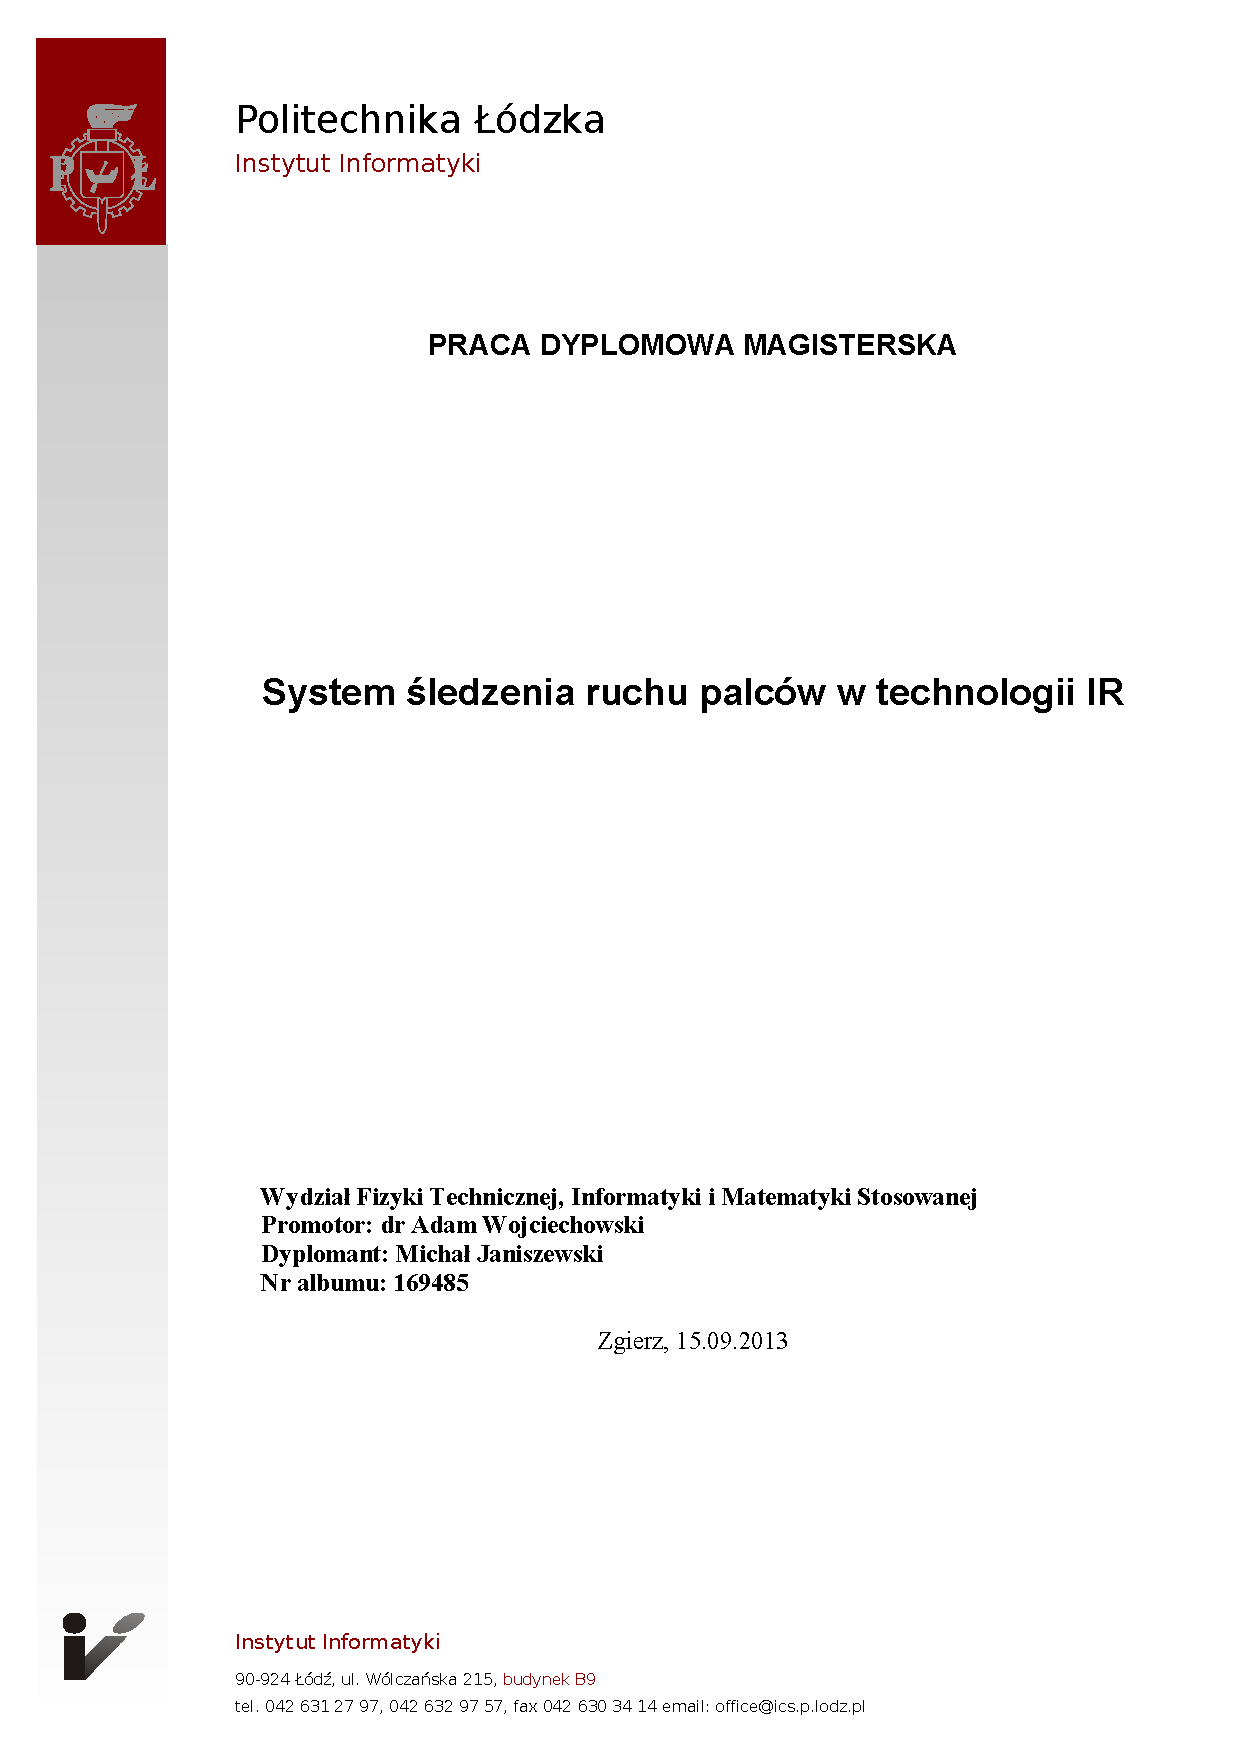
\includepdf[pagecommand={\thispagestyle{empty}}]{FrontBackmatter/front_pl.pdf}
%*******************************************************
% Titlepage
%*******************************************************
\begin{titlepage}
    % if you want the titlepage to be centered, uncomment and fine-tune the line below (KOMA classes environment)
    \begin{addmargin}[-1cm]{-3cm}
    \begin{center}
        \large
        
        \hfill
        
        \vfill
        
        \begingroup
            \color{Maroon}\spacedallcaps{\myTitle} \\ \bigskip
        \endgroup
        
        \spacedlowsmallcaps{\myName}
        
        \vfill
        
        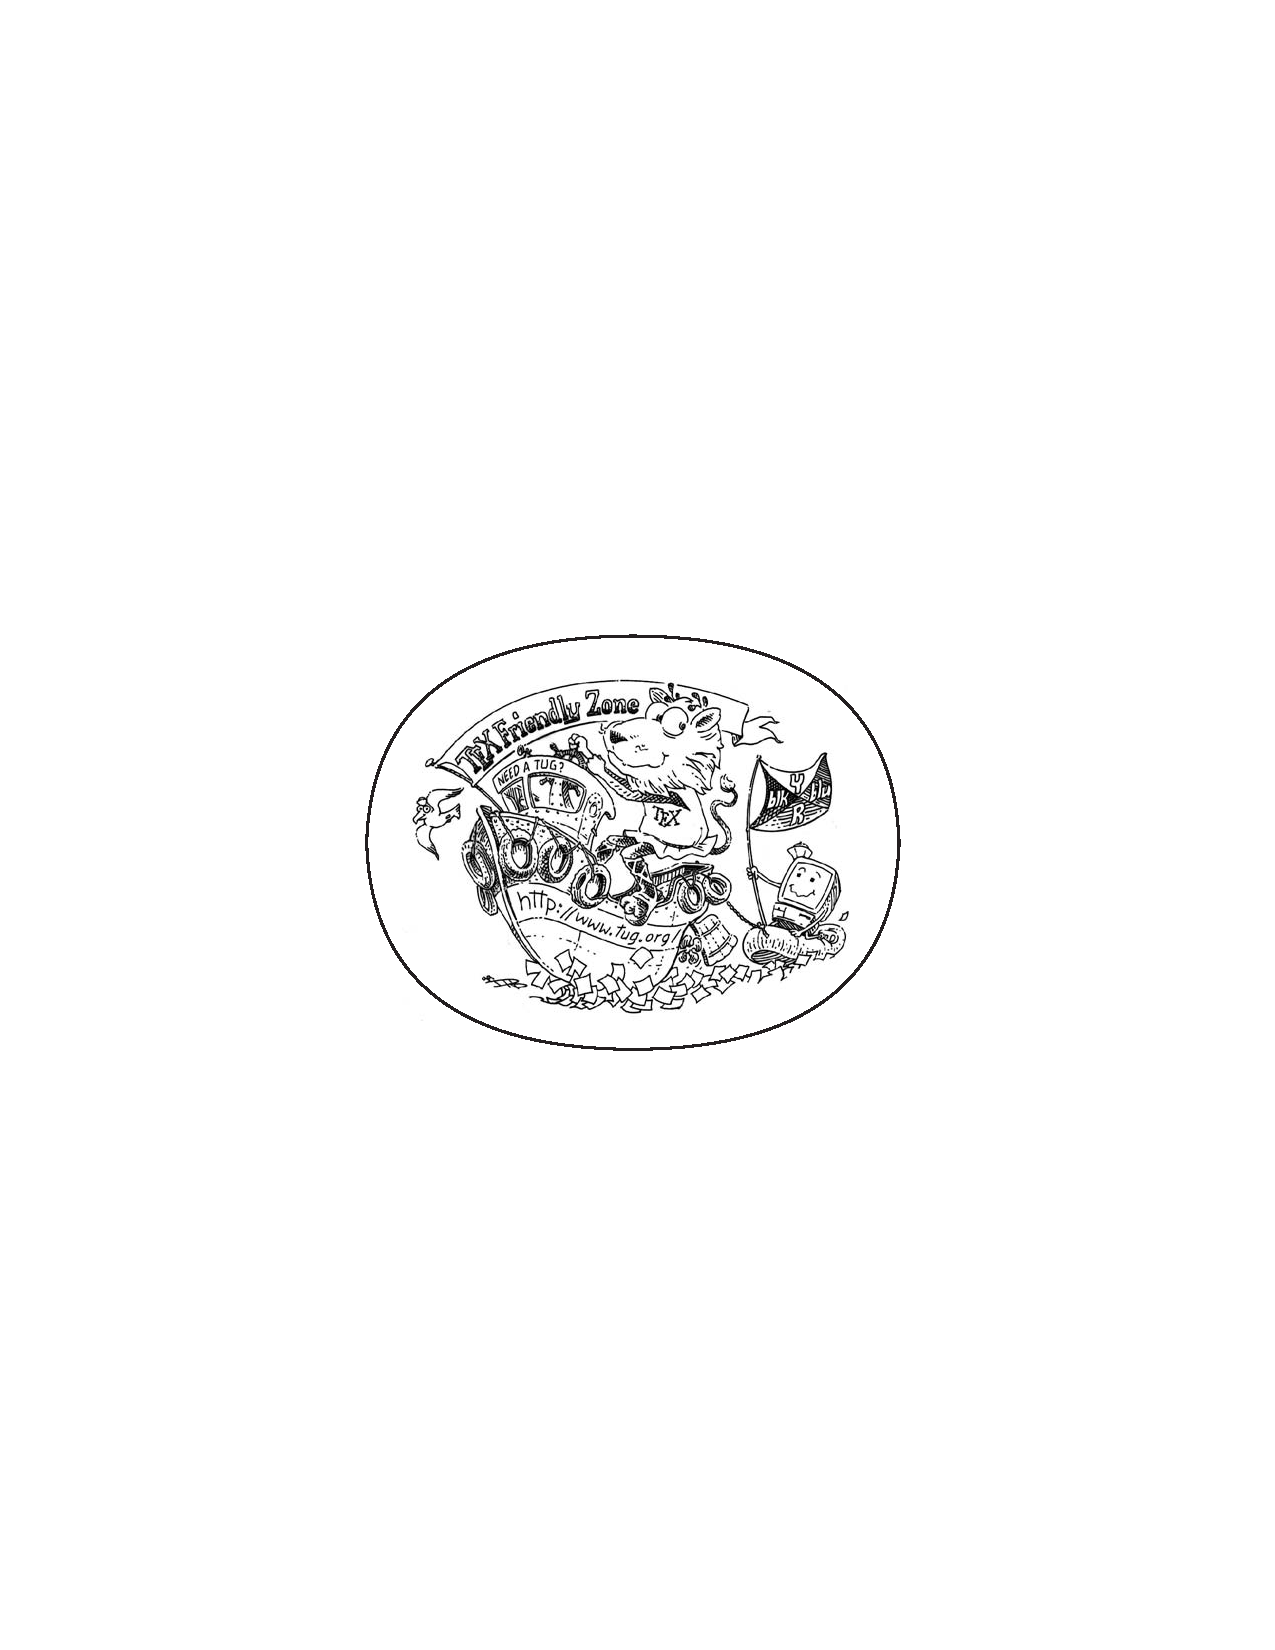
\includegraphics[width=6cm]{gfx/TFZsuperellipse_bw} \\ \medskip
        
        \mySubtitle \\ \medskip
        %\myDegree \\
        %\myDepartment \\
        %\myFaculty \\
        %\myUni \\ \bigskip
        
        \myTime\ -- \myVersion
        
        \vfill
        
    \end{center}
  \end{addmargin}
\end{titlepage}

\thispagestyle{empty}

\hfill

\vfill

\noindent\myName: \textit{\myTitle,} \mySubtitle, %\myDegree, 
\textcopyright\ \myTime

%\bigskip
%
%\noindent\spacedlowsmallcaps{Supervisors}: \\
%\myProf \\
%\myOtherProf \\ 
%\mySupervisor
%
%\medskip
%
%\noindent\spacedlowsmallcaps{Location}: \\
%\myLocation
%
%\medskip
%
%\noindent\spacedlowsmallcaps{Time Frame}: \\
%\myTime

\pagestyle{scrheadings}
%********************************************************************
% Mainmatter
%*******************************************************
\pagenumbering{arabic}
%\setcounter{page}{90}
% use \cleardoublepage here to avoid problems with pdfbookmark
\cleardoublepage
%\addtocontents{toc}{\protect\clearpage} % <--- just debug stuff, ignore
%*****************************************
\chapter{Wstęp}\label{ch:introduction}
%*****************************************

System śledzenia ruchów to pojęcie, które obejmuje szeroką gamę zestawów składających się z urządzeń dostarczających danych o położeniu oraz wyspecjalizowanego oprogramowania, które te informacje przetwarza.
Systemy takie, w ogólnym ujęciu, można spotkać w wielu miejscach:
\begin{aenumerate}
  \item w fabrykach śledzone jest przemieszczanie się produktów w celu ich dystrybucji,
  \item zarówno w produkcji gier jak i filmów stosuje się systemy \textsl{motion capture}, czyli przechwytywania ruchów,
  \item systemem śledzenia ruchów można nazwać także fotoradar przy drodze,
  \item cyfrowe modelowanie, w celu odtworzenia wirtualnego modelu istniejącego przedmiotu, często posługuje się systemem śledzenia ruchów pod postacią digitizera.
\end{aenumerate}

W każdym przypadku zarówno metoda pozyskiwania danych, protokół, którym są przekazywane oraz oprogramowanie te dane odbierające i przetwarzające jest inne, gdyż inne są wymagania, założenia i~konstrukcja każdego z tych systemów.

Spośród mnogiej ilości zastosowań takich systemów najbardziej interesującym z mojego punktu widzenia jest śledzenie ruchów na potrzeby odwzorowania ich w grach wideo.

W swojej pracy przybliżę istniejące systemy wykorzystywane w konsolach w dniu dzisiejszym oraz zaprezentuję metodę śledzenia ruchów, którą można wykorzystać do interakcji z komputerem.

%*****************************************
\chapter{Cel i założenia pracy}\label{ch:purpose}
%*****************************************

\section{Cel}

Celem pracy jest stworzenie, zademonstrowanie i ewaluacja systemu śledzenia palców przy wykorzystaniu technologi IR\graffito{IR, infrared \ppauza podczerwień.}.

W ostatnich latach przystępność komputerów znacznie wzrosła, a w ślad za tym poszedł rozwój systemów interakcji z urządzeniami cyfrowymi. Z każdą wersją sprzętu, czasami też oprogramowania, wprowadzane są coraz nowsze i nowsze metody wejściowe zacierające granice pomiędzy czynnościami związanymi z obsługą komputera, a naturalnymi ruchami.

Prym na tym polu wiodą konsole wraz z telefonami, czyli urządzenia nastawione przede wszystkim na dostarczanie rozrywki. Zaraz za nimi, skupiając się na innych aspektach, podążają metody sterowania robotami: wojskowymi, medycznymi, osobistymi. Chociaż rozwiązania z jednej dziedziny swobodnie przepływają do drugiej, to dla zwykłego użytkownika komputerów zmieniło się bardzo niewiele.

Tworzony system ma za zadanie zbadać możliwość przystosowania jednej z dostępnych metod detekcji obiektów na potrzeby komputera klasy PC.\\

\section{Założenia}

Tworzony system będzie składał się z dwóch części:
\begin{itemize}
 \item sprzętowej,
 \item programowej.
\end{itemize}

Obie te części będą ściśle pracować w tandemie, a ich przydatność osobno będzie ograniczonej wartości.

Pożądane jest, aby system pozwalał na śledzenie ruchu palców, co będzie eliminować konieczność wykorzystywania dodatkowych obiektów lub specjalizowanych narzędzi.

System ten jest znacząco różny od powszechnie dostępnych na chwilę obecną rozwiązań.

%************************************************
\myChapter{Aktualny stan zagadnienia}\label{ch:current_state}
%************************************************

Zaczynając w 2010r. swoją pracę inżynierską, jedynym dostępnym powszechnie systemem ,,alternatywnym'' systemem interakcji z komputerami, rozumianym tutaj w szerokim kontekście - t.j. także konsolami, był Wiimote firmy Nintendo - kontroler wyposażony w kamerę rejestrującą pozycję dwóch markerów świecących w podczerwieni, akcelerometr MEMS, a w póżniejszych wersjach także żyroskop MEMS. Od tego czasu, na skutek bardzo dobrego przyjęcia się takiego sposobu sterowania, szczególnie w grupie ,,\textit{casual gamers}'', nastąpił gwałtowny postęp w dziedzinie interakcji człowiek-komputer.\\

\section{Konsole}

Dzisiaj producenci konsol prześcigają się w proponowanych technologiach wykorzystywanych przede wszystkim na potrzeby rozrywki urządzeniach wejściowych:
\begin{itemize}
 \item \textsmaller{Sony PlayStation Move}, 2H2010, wykorzystuje kamerę oraz kontroler z kulą podświetlaną diodą RGB, żyroskopem, magnetometrem oraz akcelerometrem (w sumie 9 stopni swobody), kamera zawiera 4-komorowy mikrofon, który dzięki analizie czasu odebrania dźwięku, umożliwia lokalizację źródła dźwięku,
 \item \textsmaller{Microsoft Kinect}, 2H2010, oparty o dwie kamery: jedną pracującą w paśmie światła widzialnego, drugą pracującą w podczerwieni, która odczytując wzorzec świetlny nadany przez znajdujący się w urządzeniu laserowy projektor, dostarcza mapę głębokości sceny. Oprogramowanie konsoli Xbox 360 przetwarza dostarczone dane i odtwarza z nich szkielet gracza,
 \item \textsmaller{Nintendo 3DS}, 1H2011, streetpass \graffito{\color{red} to nie jest HCI, ale wpływa na użytkowanie konsoli - pisać o tym?},
 \item \textsmaller{Sony PlayStation Vita}, 1H2012, oferuje bogaty zestaw urządzeń wejściowych: żyroskop, akcelerometr, odbiornik GPS, ekran dotykowy (z przodu), panel dotykowy (z tyłu), dwie kamery,
 \item \textsmaller{Nintendo Wii U}, 2H2012, kontrolery tej konsoli zawierają dodatkowy wyświetlacz, moduł NFC\graffito{Near-field communications}, mikrofon, żyroskop, magnetometr, akcelerometr,
 \item \textsmaller{Microsoft Kinect (Xbox One)}, 2H2013, usprawniona wersja urządzenia \textsmaller{Kinect}, zawierająca kamerę type ,,time-of-flight'' badającą głębokość całej sceny w jednym przebiegu
 \item \textsmaller{Sony PlayStation 4}, 2H2013, kolejna wersja sprzętu opartego o \textsmaller{PlayStation Move} będzie zawierać dwie kamery, umożliwiając rekonstrukcję sceny w 3D, kontrolery zawierają  podświetlaną ściankę (w celu umożliwienia śledzenia ich przez kamery) oraz panel dotykowy.
\end{itemize}

Większość z wymienionych powyżej systemów opartych jest o podstawowe kontrolery zawierające przyciski, gałki, silniczki wibrujące oraz głośniki (lub możliwość podłączenia zestawu słuchawkowego), umożliwiające przesyłanie sygnałów zwrotnych z komputera dla użytkownika.

Nie należy zapominać o urządzeniach pracujących pod kontrolą systemów iOS oraz Android, których popularyzacja znacząco wpływa na dostępność urządzeń dotykowych, często z mnogością innych czujników.\\

\section{Kickstarter}

Nie tylko istniejący już producenci sprzętu rozwijają nowe technologie, od czasu powstania serwisu Kickstarter, platformy umożliwiającej finansowanie dużych przedsięwzięć osobom prywatnym przez tzw.\ \textit{crowd-funding}, z jego pomocą światło dzienne ujrzało kilka innowacyjnych projektów:
\begin{itemize}
 \item Leap Motion, kontroler wykorzystujący dwie kamery oraz diody podczerwone do oświetlania ,,sceny'', dostarczany z oprogramowaniem umożliwiającym śledzenie ruchów rąk,
 \item Oculus Rift, HMD\graffito{Head-mounted Display} z zestawem czujników umożliwiający swobodne rozglądanie się w świecie gry,
 \item Mycestro, zakładane na palec urządzenie zastępujące mysz, wykorzystujące 3-osiowy żyroskop oraz czyjnik dotykowy,
 \item TouchKeys, nakładki dotykowe na klawisze pianina.\\
\end{itemize}

\section{Inne}

Jednym z bardziej interesujących projektów, którego nie można uwzględnić w powyższych listach jest \textsmaller{Myo}, opaska zakładana na rękę odczytująca sygnały elektryczne płynące do mięśni, wykrywająca ruchy ,,u źródła''.

Wymienione powyżej, to tylko niektóre ze sfinansowanych projektów, pokazują jednak one trend dążący do usprawnienia metod komunikacji z komputerem. Cechą wspólną ich wszystkich jest usunięcie bariery, jaką stanowi wprowadzanie danych do urządzeń cyfrowych - sprawienie, aby komputery stały się niedostrzegalne dla użytkownika, który podczas codziennych czynności nie będzie zastanawiał się w jaki sposób zmusić komputer do działania. Odpowiedzialność zostanie przełożona na komputer, którego zadaniem będzie interpretacja zamiarów człowieka i wspomożenie go wtedy, gdy zajdzie potrzeba.

Znaczący postęp w tej dziedzinie, jaki miał miejsce na przestrzeni ostatnich kilku lat, oraz związane z nim zwiększenie popularności tego typu urządzeń oraz wsparcia ze strony sprzętu i oprogramowania zachęca do podejmowania dalszych prób, eksperymentów, które można już wykonywać w zaciszu domowym.

%************************************************
\myChapter{Sprzęt}\label{ch:hardware}
%************************************************

Na potrzeby realizacji pracy wymagane było stworzenie sprzętu \pauza urządzenia wejściowego, które będzie pozwalało na śledzenie ruchów palców użytkownika.

Podczas projektowania powstało kilka dodatkowych założeń, które sprzęt powinien spełniać:
\begin{itemize}
 \item łatwość podłączenia \pauza urządzenie powinno być możliwe do ,,zainstalowania'' w kilka chwil, najlepiej bez konieczności korzystania z narzędzi, podłączania zbyt wielu przewodów,
 \item łatwość użytkowania \pauza urządzenie powinno umożliwiać interakcję z komputerem osobom niezapoznanym z pracą, niekoniecznie posiadającym wiedzę techniczną dotyczącą zasady działania,
 \item działanie w możliwie najróżniejszych warunkach \pauza uwzględnienie spodziewanych warunków pracy urządzenia, tak aby nie przeszkadzały one w jego użytkowaniu,
 \item prostota i modułowość \pauza zmniejszenie kosztów produkcji poprzez zastosowanie możliwie prostych, dostępnych i sprawdzonych części połączonych w łatwo wymienialne moduły, co dodatkowo poprawi możliwość zastępowania elementów w wypadku ich uszkodzenia.\\
\end{itemize}

Urządzenie składa się z aluminiowej ramy, złożonej z czterech kątowników, z wywierconymi otworami na diody, fotodiody i elementy mocowania. Rama została zaprojektowana, aby pasowała do posiadanego monitora o przekątnej 24''.

\section{Moduły}

Do ramy przymocowanych jest 20 modułów \pauza po 4 na krótsze i po 6 na dłuższe boki.

Każdy z jednakowych modułów zawiera:
\begin{itemize}
 \item diodę emitującą światło w paśmie podczerwieni (TSAL6400),
 \item 8 fotodiod reagujących na światło wymienionej wyżej diody,
 \item ośmioportowy trzystanowy bufor (74LS541),
 \item zestaw złącz, oporników wymaganych do funkcjonowania powyższych elementów.
\end{itemize}

Moduły połączone zostały ośmiokanałowym interfejsem równoległym, dodatkowo z dwiema żyłami niosącymi zasilanie oraz osobnymi przewodami z sygnałami chip select (\textsmaller{\textoverline{CS}}) dla bufora oraz diody świecącej (\textsmaller{CS}).\\

Odstęp pomiędzy fotodiodami wynosi 10mm, natomiast między nadajnikami 80mm, co przekłada się na charakterystykę modułów: 8 odbiorników w równych odstępach, 1 nadajnik po środku.
Średnica odbiorników wynosi 3mm, zaś nadajników:
\begin{itemize}
 \item w pierwotnym planie też 3mm, rozmieszczone jeden nad drugim w celu zwiększenia ich widoczności,
 \item w finalnej wersji jeden nadajnik o średnicy 5mm.\\
\end{itemize}

Dodatkowo, nadajniki przesunięte są o 5mm względem rastra wyznaczonego przez odbiorniki, tak aby znajdowały się idealnie pomiędzy fotodiodami.

Moduły zostały zaprojektowane w taki sposób, aby rozmieszczenie fotodiod i nadajników było jednolite, bez względu na granice między modułami. Każdy moduł posiada 4 dodatkowe otwory służace przymocowaniu ich do ramki za pomocą śrub.\\

Otwory na moduły wiercone były w miękkim aluminium wykorzystując wzorzec ze stali, którego wykonanie zostało zlecone zewnętrznej firmie.
Wzorzec ten zawierał otwory nie tylko dla jednego modułu (nadajniki, odbiorniki, elementy mocowania), ale także dwa elementy mocujące poprzedniego modułu, co pozwalało na wygodną synchronizację otworów podczas wiercenia. Wzorzec przedstawiony jest na rysunku \ref{fig:holes_master}. Po prawej stronie widać dwa otwory synchronizacyjne (górny \ppauza montażowy, dolny \ppauza fotodioda), u góry po środku otwory nadajników.\\

\begin{figure}
 \centering
 \makebox[\textwidth][l]{
  \resizebox{.9\largefigure}{!}{
    \def\svgwidth{0.9\largefigure}
    \includesvg{gfx/holes_master}
  }
 }
 \caption{Wzorzec do wiercenia otworów.}
 \label{fig:holes_master}
\end{figure}

Dwie płytki drukowane, każda z zestawem układów 74HC4514 i 74HC4515, pełnią funkcję demultipleksera portów \pauza układy te to dekodery 4\ppauza{}do\ppauza{}16 z zapadkami (\textsl{latches}), które umożliwiają komunikację z modułami za pomocą znacznie zredukowanej ilości pinów niż byłaby wymagana, gdyby każdy moduł podłączać bezpośrednio.
Zastosowanie takiego rozwiązania jest szybsze niż w przypadku interfejsu szeregowego, np. takiego jak I\textsuperscript{2}C lub SPI, jednak pociąga za sobą konieczność poprowadzenia sygnału \textsmaller{CS} oraz \textsmaller{\textoverline{CS}} do każdego modułu osobno zamiast zintegrowania go w magistrali łączącej wszystkie moduły wygodną do podłączania tasiemką.
Konieczność instalowania w każdym module dekodera takiego interfejsu, ustawiania adresów logicznych modułów, chociaż pozwalałaby na dalsze rozszerzanie ramki o kolejne moduły, zwiększałaby koszty oraz wymagany nakład pracy, rozumianej zarówno przez tworzone oprogramowanie jak i ,,koszt'' działania programu, tj. czasu wymaganego do obsługi wybranego protokołu, zaważyły o ostatecznym wyborze rozwiązania równoległego.

Wszystkie płytki PCB\graffito{PCB, printed circuit board \ppauza płytka z układem drukowanym.}, z wyjątkiem modułu mikrokontrolera, zostały zaprojektowane i wykonane wyłącznie w celu realizacji pracy.

Stworzony sprzęt przeszedł kilka zmian: zarówno mikroprocesor jak i elementy konstrukcji były kilkukrotnie wymieniane.\\

\section{Rewizja pierwsza}

W pierwszej wersji do kontroli modułów i interfejsowania z komputerem wykorzystany został mikrokontroler z 16-bitowej rodziny MSP430: MSP430FG4618 znajdujący się w płytce Experimenter's Board.
Pod kątem tego urządzenia projektowane były wszystkie interfejsy, uwzględniając przede wszystkim ilość dostępnych pinów oraz charakterystykę prądową.
Płytkę tę prezentuje rysunek~\ref{fig:msp430_exp}.

\begin{figure}
%  \centering
%  \makebox[\textwidth][r]{
%   \resizebox{.9\largefigure}{!}{
%   }
%  }
 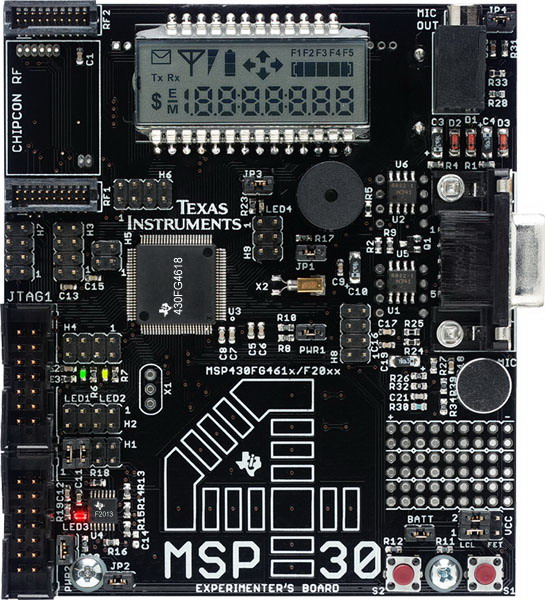
\includegraphics[width=\textwidth]{gfx/exp43000}
 \caption{Płytka MSP430 experimenter's board.}
 \label{fig:msp430_exp}
\end{figure}

\begin{figure}
 \centering
 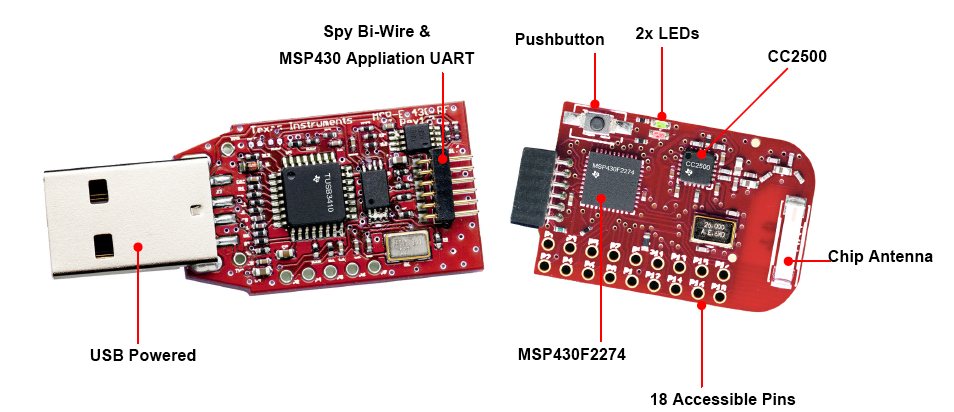
\includegraphics[width=\textwidth]{gfx/ez430-rf2500}
 \caption{Płytka MSP430 eZ430-rf2500}
 \label{fig:msp430_ez430}
\end{figure}

Duże problemy okazał się powodować moduł komunikacji szeregowej UART, który operował w standardzie RS232/TTL\graffito{TTL, transistor\ppauza{}to\ppauza{}transistor logic, poziomy napięć i prądów przystosowane do niedługich połączeń pomiędzy układami}.
Po podłączeniu adaptera USB\ppauza{}RS232 opartego o renomowany układ FTDI FT2232C okazało się w testach, że podczas dużego obciążenia hosta, pojedyncze bity ramki RS232 mogą się ,,zgubić'', tj. jedynki sporadycznie zastępowane były zerami.
Ze względu na spodziewany charakter wykorzystywania pracy, np. podczas gier, oczekiwane było poprawne działanie także w warunkach wysokiego obciążenia, co dyskwalifikowało takie rozwiązanie.\\

\section{Rewizja druga}

Z powodu dostępności płytki eZ430-RF2500 chciałem wykorzystać zawarty na niej układ MSP430F2274, który mógłby zapewnić spodziewaną stabilność transmisji danych.
Płytka ta podłączana była do komputera bezpośrednio do portu USB, co pozwalało przypuszczać, że wykorzystując inny, znacznie nowszy, podsystem komputera, będzie on działał poprawnie.
Pomimo przeprojektowania płytki interfejsu ramka $\leftrightarrow$ mikrokontroler, która ograniczała liczbę wymaganych połączeń z 24 do 20 \pauza możliwie najniższej praktycznie osiągalnej ilości niewymagającej połączeń szeregowych, układ nie miał nawet takiej ilości złącz GPIO\graffito{GPIO, general-purpose input/output, \pauza interfejs wejścia/wyjścia}.
Ponadto prędkość transmisji była sztucznie ograniczona do wartości 9600BPS, która nie zapewnia wymaganej przepustowości.

Płytkę widać na rysunku~\ref{fig:msp430_ez430}.\\

\section{Rewizja trzecia}

Ze względu na problemy z komunikacją, zdecydowałem się wykorzystać do pracy nowy układ z rdzeniem ARM Cortex\ppauza{}M4F, Texas Instruments LM4F120H5QR na płytce Stellaris Launchpad. Jest to 32-bitowy procesor, dostępny dopiero od listopada 2012, tj. kilka miesięcy po rozpoczęciu pisania pracy.
Układ ten posiada zintegrowany kontroler urządzenia USB pozwalający na uzyskanie niezawodności komunikacji na zadowalającym poziomie.
Moduł pokazany jest na rysunku~\ref{fig:stellaris_launchpad}.

\begin{figure}
 \centering
 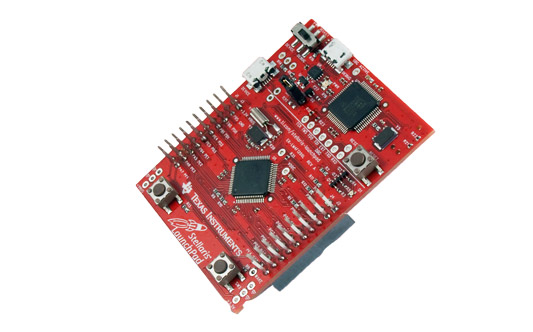
\includegraphics[width=\textwidth]{gfx/stellaris_launchpad}
 \caption[Płytka Stellaris Launchpad]{Płytka Stellaris Launchpad z układem TI LM4F120H5QR}
 \label{fig:stellaris_launchpad}
\end{figure}

Dopiero uzyskanie tego układu pozwoliło na dalszy postęp prac. Problemy związane z brakiem odpowiedniego sprzętu i funduszy na zakup mocniejszych układów były główną przyczyną rozciągnięcia się pracy w czasie.\\

\section{Rewizja czwarta}

W tej wersji, zmieniona została konstrukcja samej ramki i modułów. Pierwotny projekt zakładał, że diody emitujące światło znajdować będą się w innej płaszczyżnie niż elemnty odbiorcze w celu uniknięcia problemu odbić. Moc wykorzystanych wtedy diod okazała się niewystarczająca do poprawnego oświetlenia odbiorników, przesunięte zostały więc one do płaszczyzny odbiorników.

Z powodu nadal niedostatecznej ilości mocy diod, wymienione zostały na modele 5\texttimes\  mocniejsze, używające 120mA: TSAL6400. Dodane także zostały (do niektórych modułów) diody świecące w paśmie światła widzialnego, element nieprzewidziany w pierwotnym projekcie, co pozwoliło na prostsze debugowanie działania urządzenia.\\

\section{Interfejs ramka $\leftrightarrow$ mikrokontroler}

Interfejs zapewniający komunikację pomiędzy mikrokontrolerem, a ramką przeszedł tylko jedną wymianę, mającą na celu przede wszystkim wspomniane już ograniczenie ilości wymaganych pinów do obsługi.

Pierwsza wersja oparta była na układach 74LS139 (podwójny selektor 1\ppauza{}z\ppauza{}4) oraz 74LS14 (inwerter), posiadała także zestaw diod LED i oporników pomocnych w debugowaniu. Działanie tego urządzenia było bardzo proste, polegało na wyborze odpowiedniego modułu (nadawczego i odbiorczego) poprzez ustawienie sygnałów \textsmaller{CS} oraz \textsmaller{\textoverline{CS}} po wybraniu danego układu oraz ,,wysłania'' do niego adresu jednej z czterech linii wyjściowych. Sygnał \textsmaller{\textoverline{CS}} uzyskany został przez zastosowanie inwertera 74LS14.

Płytkę tę przedstawia rysunek~\ref{fig:first_interface}.
Na tym rysunku płytka jest rozłączona.\\

Druga, a zarazem finalna wersja tego sprzętu wykorzystuje w tym celu dwie płytki PCB, każda zawierająca po jednym układzie 74HC4514 oraz 74HC4515. Układy te to selektory 1\ppauza{}z\ppauza{}16, które różnią się tylko i wyłącznie wbudowanym inwerterem: 74HC4514 posiada wolną jedynkę, tzn. na wybranym wyjściu ustawiony zostanie stan wysoki, pozostałe linie mają stan niski; układ 74HC4515 posiada wolne zero \pauza na każdej linii znajduje się inwerter.

Ta płytka, podobnie jak jej poprzednia wersja, zawiera zestaw diod LED umożliwiających debugowanie.

Rysunek~\ref{fig:second_interface} przedstawia drugą wersję płytki interfejsowej. Płytka ta na zdjęciu jest podłączona.\\

\begin{figure}
 \centering
 \makebox[\textwidth][l]{
  \resizebox{.8\largefigure}{!}{
   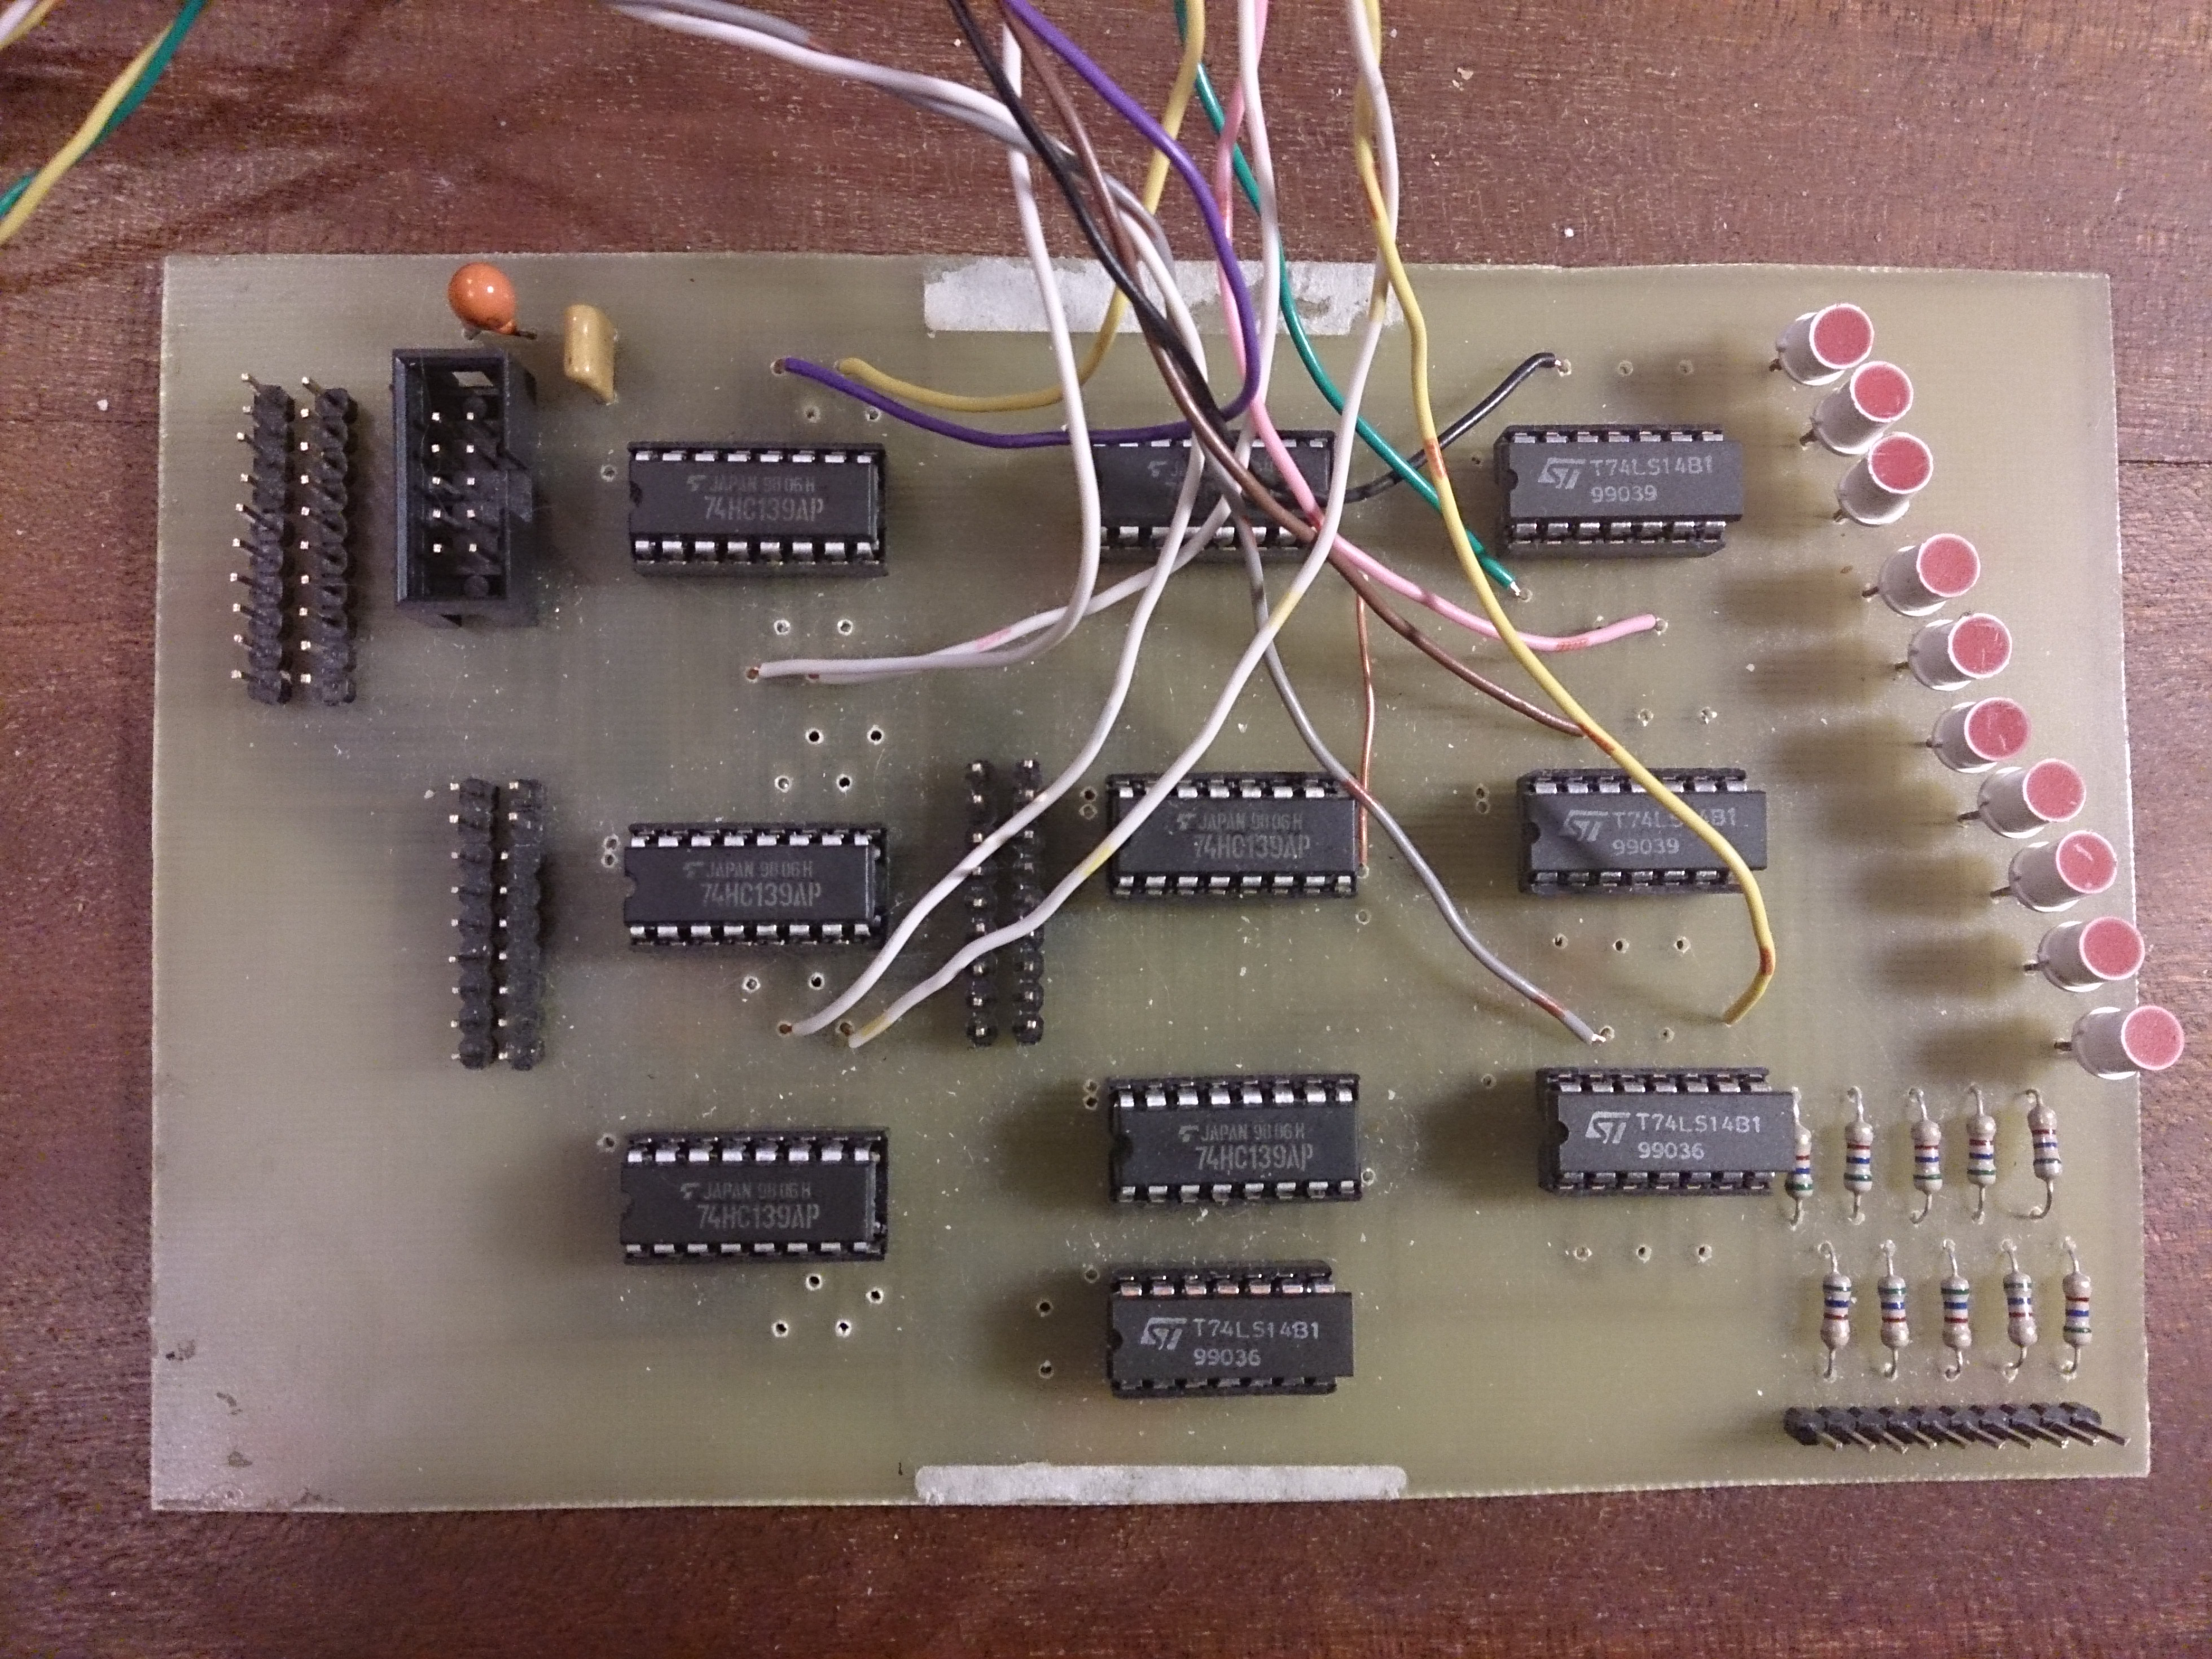
\includegraphics[width=\textwidth]{gfx/first_interface}
  }
 }
 \caption[Pierwsza wersja płytki interfejsowej]{Pierwsza wersja płytki interfejsowej (rozłączona).}
 \label{fig:first_interface}
\end{figure}

\begin{figure}
 \centering
 \makebox[\textwidth][l]{
  \resizebox{.8\largefigure}{!}{
   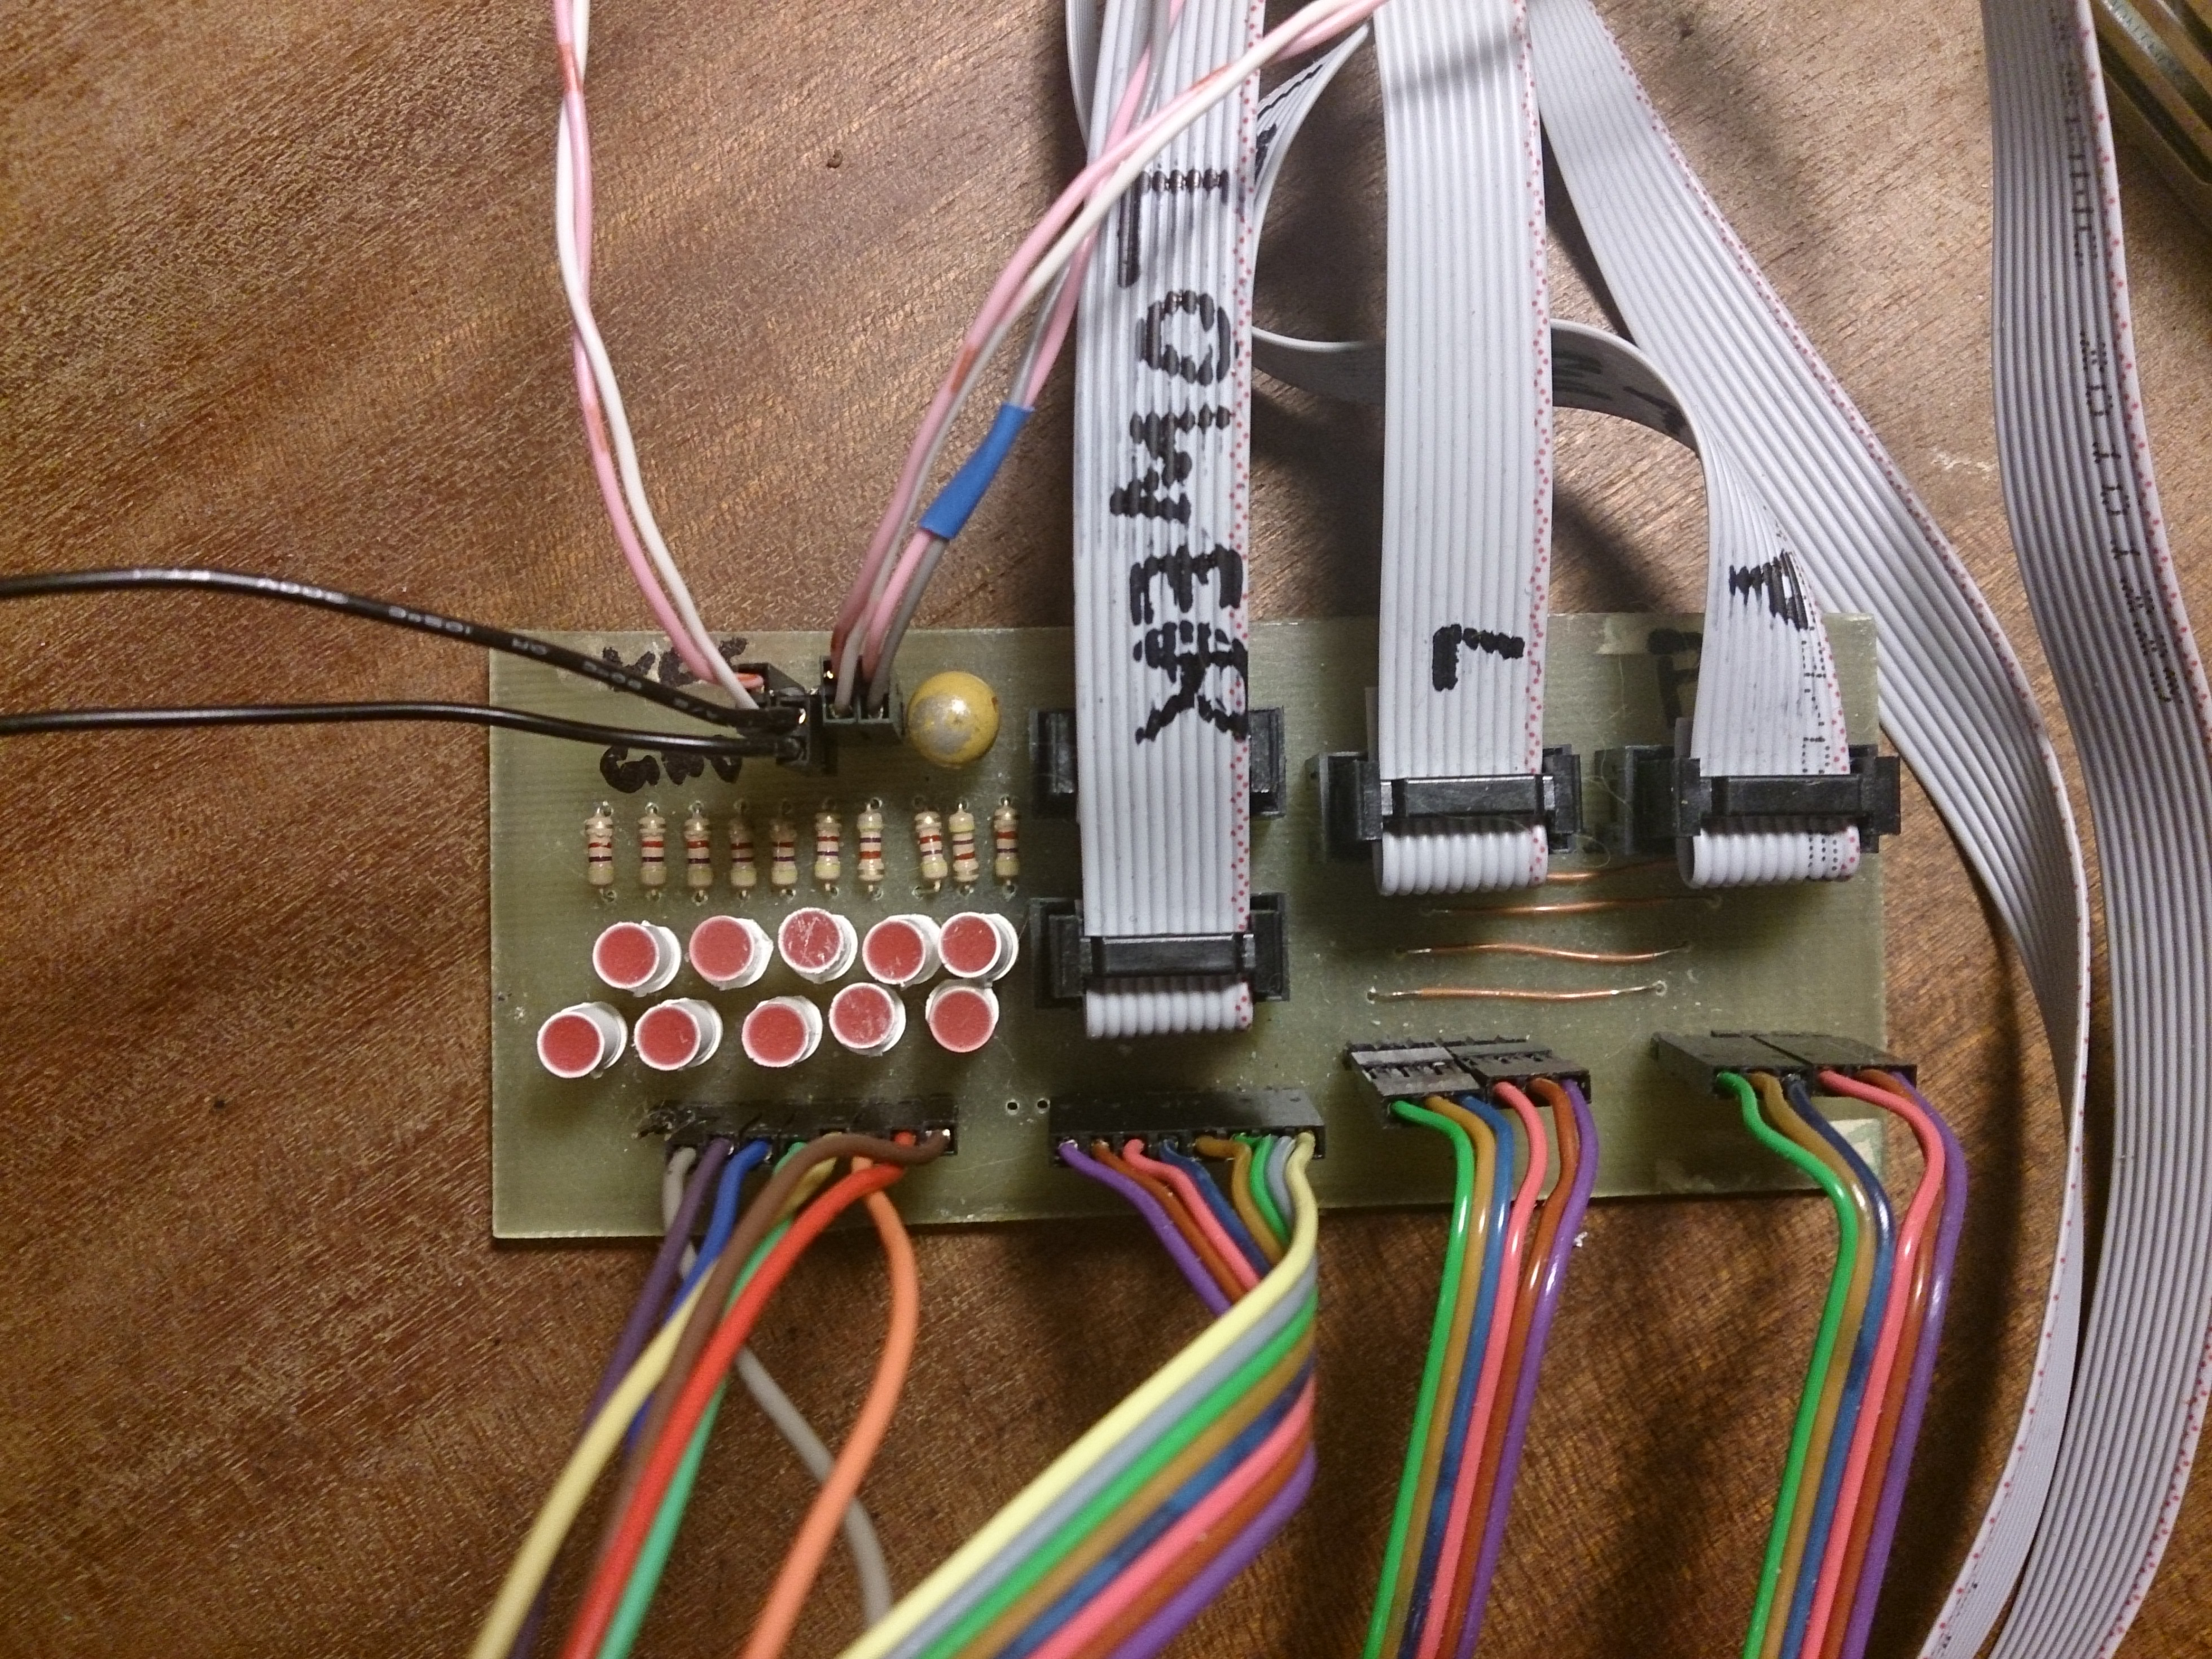
\includegraphics[width=\textwidth]{gfx/second_interface}
  }
 }
 \caption[Druga wersja płytki interfejsowej]{Druga wersja płytki interfejsowej (podłączona).}
 \label{fig:second_interface}
\end{figure}

Zastosowanie dwóch selektorów 16-liniowych wymaga sześciu linii: 4 linie adresowe oraz po jednej linii \textsmaller{\textoverline{I}} (\textsmaller{\textoverline{Inhibit}}) dla każdego układu.
Chociaż 20 użytych modułów można zaadresować za pomocą 5\ppauza{}bitowej przestrzeni adresowej zdolnej do obsługi maksymalnie 32 odbiorników, to należy zwrócić uwagę, że dekodery 5\ppauza{}do\ppauza{}32 nie istnieją.
Ich konstrukcja, choć trywialna, dodawałaby zbędnego skomplikowania oraz kosztów, dając w zamian niewiele.
Dodatkowo, posiadanie dedykowanych linii wybierających pozwala na przełączenie urządzenia w tryb ,,stand-by'', co w tym wypadku oznacza wyłączenie zarówno nadawania jak i odbierania.
Podwójne elementy sterujące umożliwiają także ograniczenie długości potrzebnych przewodów, rozmiarów płytki (ze względu na zmniejszoną ilość wyjść) oraz konieczność mniejszej ingerencji w urządzenie w razie awarii.\\

Ramkę w całej okazałości, zamontowaną na wzorcowym monitorze pokazuje rysunek~\ref{fig:frame_full}.

\begin{sidewaysfigure}[tbh]
  \myfloatalign
  \vspace{0.1\textheight}
  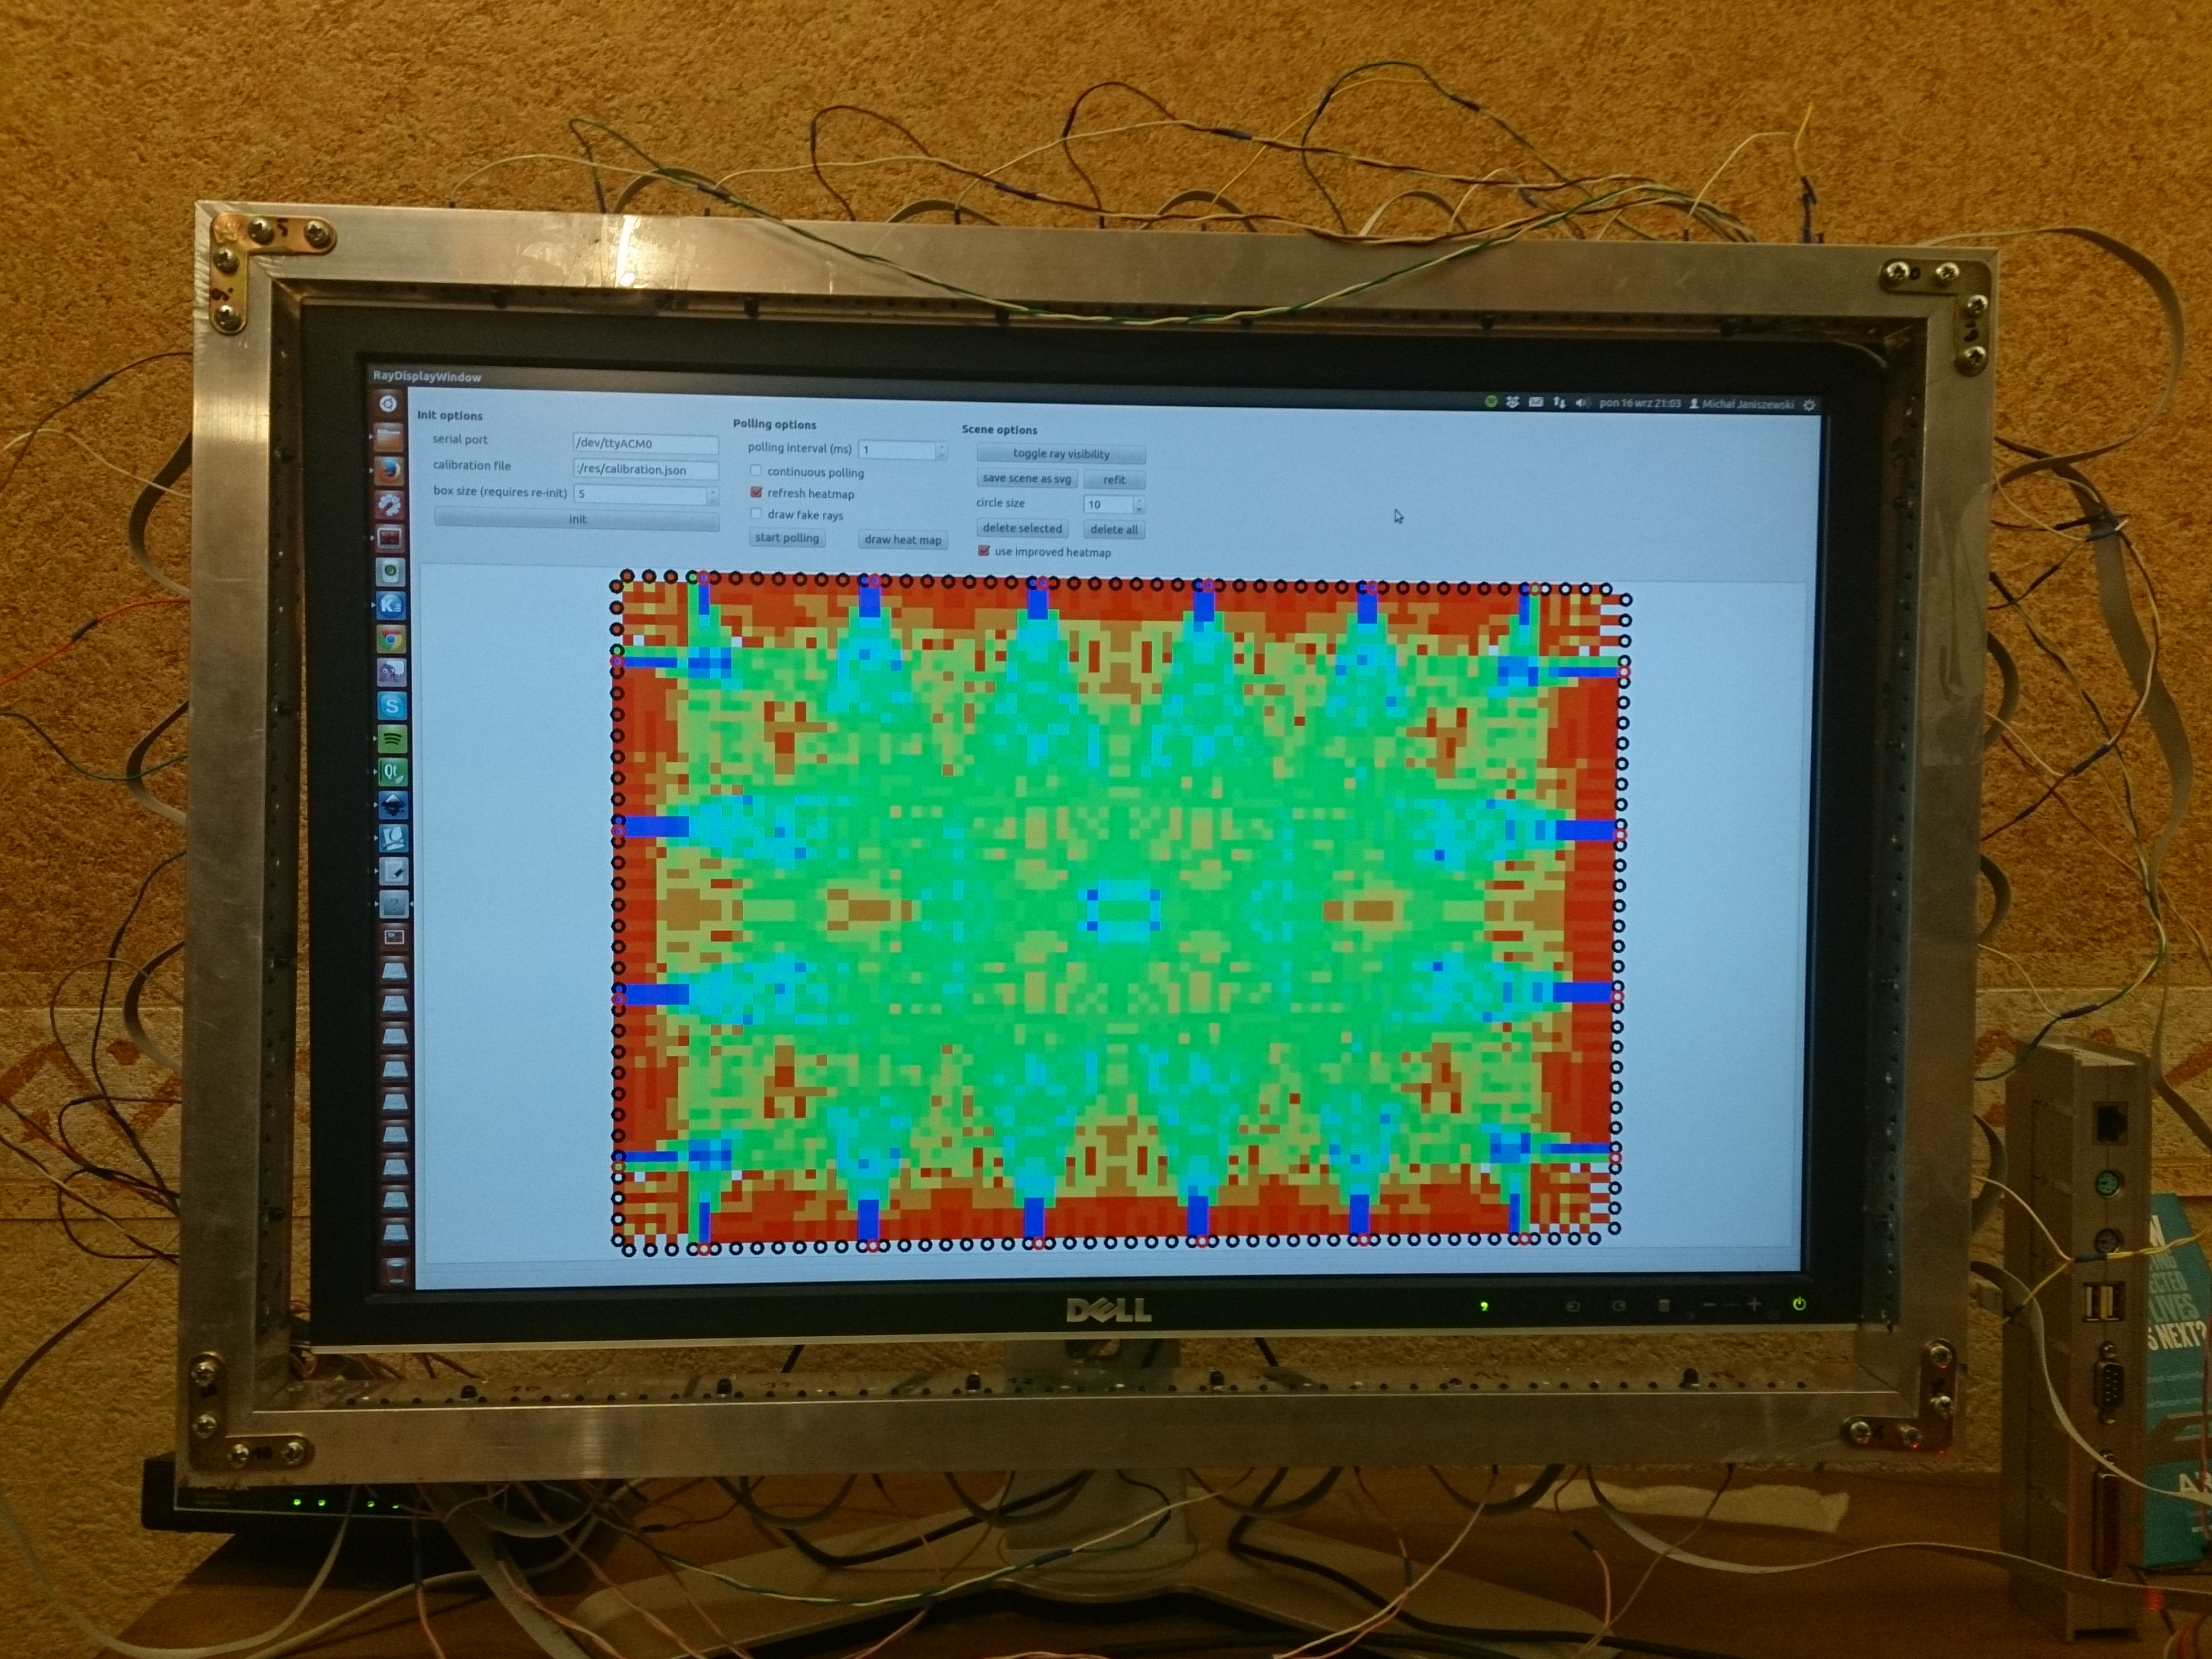
\includegraphics[width=\textwidth]{gfx/frame_full}
  \caption{Ramka zamontowana na docelowym monitorze.}
  \label{fig:frame_full}
\end{sidewaysfigure}

%************************************************
\myChapter{Metoda}\label{ch:method}
%************************************************

W tym rozdziale przedstawię metodę wykorzystaną do określania pozycji obiektów znajdujących się w ramce.\\

Ramka składa się z dwudziestu modułów, każdy z nich zawiera jedną diodę LED oraz 8 fotodiod.\\

\section{Pobieranie danych}

Podczas działania urządzenia zapalane są kolejno moduły ponumerowane od 0 do 19, układ jest zaprojektowany w taki sposób, aby w dowolnej chwili świecił się najwyżej jeden moduł. W czasie świecenia wybierane są moduły leżące po przeciwnej stronie i odczytywany jest ich stan, który następnie trafi do komputera. Host decyduje o tym które moduły należy zapalić, odpytać oraz w jakiej kolejności to zrobić. Mikrokontroler jest jednostką wykonawczą tych poleceń i dostarcza z powrotem dane w postaci wygodnej do analizy.

Na potrzeby pracy przyjmijmy, że światło z nadajnika rozchodzi się w postaci dyskretnych promieni \pauza wiązek światła łączących go z odbiornikami. Pozwala to na uproszczenie opisu metody działania bez poświęcania dokładności \pauza światło, które nie trafia w aktywną w danej chwili fotodiodę nie jest brane pod uwagę.

Przerwanie któregokolwiek z takich promieni poprzez zasłonięcie odbiornika powoduje zmianę stanu na jego wyjściu. Fotodiody oświetlone dają na wyjściu stan niski, zaś nieoświetlone \ppauza wysoki.\\

\section{Model}

Rysunek~\ref{fig:scene_rays_sample} prezentuje schemat ramki z włączonym jednym modułem. Zachowane są proporcje względem ilości modułów na ściankach oraz rozmieszczenia fotodiod w modułach względem nadajników, chociaż fizyczne wymiary urządzenia i wynikające z tego ograniczenia zostały pominięte:
\begin{itemize}
 \item odstęp pomiędzy ścianką ramki, a najbliższym modułem,
 \item wielkość fotodiod i nadajników,
 \item rozmieszczanie elementów w osi $Z$,
 \item elementy konstrukcyjne ramki (aluminiowe kątowniki, śrubki, przewody, itp.),
 \item diody LED działające w paśmie światła widzialnego.
\end{itemize}

Pominięte aspekty mają znaczenie jedynie w czytelności prezentacji i nie wpływają na poprawność przedstawianego modelu.

\begin{figure}
 %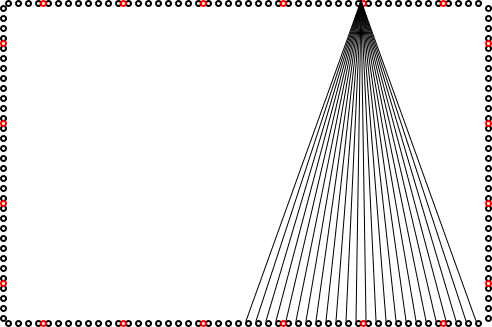
\includegraphics[width=\textwidth]{gfx/scene_rays_sample.svg}
 \centering
 \makebox[\textwidth][r]{
  \resizebox{.9\largefigure}{!}{
    \def\svgwidth{0.9\largefigure}
    \includesvg{gfx/scene_rays_sample}
  }
 }
 \caption{Wizualizacja ramki. Czarne okręgi \ppauza fotodiody; czerwone \ppauza diody LED; czarne odcinki \ppauza odbierane promienie.}
 \label{fig:scene_rays_sample}
\end{figure}

Dane o promieniach zbierane są przez mikrokontroler, opakowywane w ramki protokołu, przesyłane do komputera i po rozpakowaniu poddawane dalszemu przetwarzaniu.\\

\section{Heatmapa}

Wykorzystując te informacje można stworzyć \textit{heatmapę} prezentującą w graficzny sposób rozkład gęstości przecięć promieni zasłoniętych. Daje to możliwość wizualnego rozpoznania konturów obiektów znajdujących się wewnątrz ramki.

Wygodnym sposobem wyboru kolorów heatmapy jest wykorzystanie modelu barw HSL, przy czym wielkościom $s$ i $l$ zostały przypisane stałe wartości: $s = 1$, $l = 0.5$, natomiast parametr $h$ został dobrany w taki sposób, aby zmieniał się od $240^{\circ}$ (niebieski) do $0^{\circ}$ (czerwony) i reprezentował tym odpowiednio ,,mało'' i ,,dużo'', przy czym dokładne wartości ze skali nie mają istotnego znaczenia, a jedynie ich względna wielkość.

Heatmapa generowana jest w następujący sposób:
\begin{enumerate}
 \item Scena, wnętrze reprezentacji ramki na komputerze, dzielona jest na kwadraty $A_{x,y}$ o zadanym boku $a$, a każdemu z nich przyporządkowywany jest licznik $C$ z początkową wartością $C_{i,j} = 0$,
 \item pobierane kolejno są dane o zasłoniętych promieniach dla każdego z modułów,
 \item dla każdego zasłoniętego promienia wyznaczany jest \textit{bounding box}, z dokładnością do $a$,
 \item dla każdego kwadrata z bounding boksa promienia sprawdzane jest, czy promień przechodzi przez ten kwadrat, tj. czy przecina którąkolwiek z jego ścianek,
 \item jeśli promień przecina kwadrat $A_{i,j}$, to wartość jego licznika $C_{i,j}$ jest inkrementowana o $1$,
 \item po przetworzeniu wszystkich aktualnie dostępnych danych, znajdowana jest największa wartość licznika $C$, $C_{max}$, względem której skalowane są kolory heatmapy,
 \item dla każdego kwadrata $A_{i,j}$, jeśli $C_{i,j} > 0$, rysowany jest w scenie kwadrat o wyznaczonym kolorze.
\end{enumerate}

Wybrane kroki powyższego algorytmu prezentują rysunki \ref{fig:scene_intersections}, \ref{fig:scene_rays}, \ref{fig:scene_heatmap} oraz \ref{fig:scene_heatmap_overlay}.

\begin{sidewaysfigure}[tbh]
  \myfloatalign
  \subfloat[Wizualizacja sceny wraz z jednym promieniem, bounding boksem i wybranymi przecinanymi kwadratami]
  {\label{fig:scene_intersections}
  \def\svgwidth{0.47\linewidth}
  \includesvg{gfx/scene_intersections}} \quad
  \subfloat[Wizualizacja sceny z przykładowymi promieniami]
  {\label{fig:scene_rays}%
  \def\svgwidth{0.47\linewidth}
  \includesvg{gfx/scene_rays}} \\
  \subfloat[Wizualizacja sceny z heatmapą]
  {\label{fig:scene_heatmap}
  \def\svgwidth{0.47\linewidth}
  \includesvg{gfx/scene_heatmap}} \quad
  \subfloat[Wizualizacja sceny z heatmapą i nałożonymi promieniami]
  {\label{fig:scene_heatmap_overlay}
  \def\svgwidth{0.47\linewidth}
  \includesvg{gfx/scene_heatmap_overlay}}
  \caption[Algorytm konstrukcji heatmapy]{Algorytm konstrukcji heatmapy, $a$ = 10.}\label{fig:scene_heatmap_algorithm}
\end{sidewaysfigure}

Ze względu na możliwość badania jedynie obecności lub braku promienia, system jest w stanie raportować w najlepszym przypadku otoczkę wypukłą obiektów. Otoczka wypukła zbioru punktów $A$, oznaczana zwykle $\mbox{conv} A$ to najmniejszy wypukły zbiór punktów zawierający $A$.\\

\clearpage

Na potrzeby testów i prezentacji stworzyłem dodatkową funkcjonalność pozwalającą na rozmieszczanie w scenie wirtualnych przeszkód, pozwala to przedstawić działanie algorytmów w pewnej teoretycznej, idealnej sytuacji, która nie zawsze występuje przy rozwojowym sprzęcie.

Większość przedstawianych w tym rozdziale sytuacji będzie opierać się o fikcyjne przeszkody pod postacią okręgów.\\

Wykorzystując opisany wcześniej algorytm generowania heatmapy można już zaimplementować system wykrywania przeszkód. Istotnym dla działania programu jest wybór wielkości $a$. Mniejsze wartości zwiększają rozdzielczość kosztem większej ilości danych do przetworzenia, zaś większe mogą zapewnić mniejszą podatność na szumy (fałszywe pozytywy i negatywy). Wpływ wielkości $a$ na algorytm konstruujący heatmapę prezentuje rysunek~\ref{fig:scene_heatmap_size}.

\begin{sidewaysfigure}[tbh]
  \myfloatalign
  \subfloat[$a$ = 5]
  {\label{fig:scene_heatmap_5}
  \def\svgwidth{0.46\linewidth}
  \includesvg{gfx/scene_heatmap_5}} \quad
  \subfloat[$a$ = 10]
  {\label{fig:scene_heatmap_10}%
  \def\svgwidth{0.46\linewidth}
  \includesvg{gfx/scene_heatmap_10}} \\
  \subfloat[$a$ = 15]
  {\label{fig:scene_heatmap_15}
  \def\svgwidth{0.46\linewidth}
  \includesvg{gfx/scene_heatmap_15}} \quad
  \subfloat[$a$ = 20]
  {\label{fig:scene_heatmap_20}
  \def\svgwidth{0.46\linewidth}
  \includesvg{gfx/scene_heatmap_20}}
  \caption[Wpływ wielkości $a$ na algorytm konstrukcji heatmapy.]{Wpływ wielkości $a$ na algorytm konstrukcji heatmapy.}\label{fig:scene_heatmap_size}
\end{sidewaysfigure}


Jak widać, dla małych wartości $a$, miejsca przecięć promieni zakrytych wartość licznika $C$ jest niewiele większa od wartości w okolicach nadajników, gdzie zbiega się wiele promieni. Wraz ze zwiększaniem $a$ charakterystyka heatmapy zmienia się na rzecz lepszego uwidocznienia zasłaniającego obiektu, jednak maleje przy tym dostępna rozdzielczość wykrywania.\\

\section{Ulepszona heatmapa}

Problem małych wielkości licznika $C$ rozwiązałem ulepszając pierwotny algorytm generowania heatmapy wykorzystując także dane o prawdziwych negatywach, tj. promieniach, o których wiadomo, że powinny być widoczne, jeśli nie napotkały na przeszkodę.

Ulepszony algorytm wygląda następująco (zmiany zostały wyróżnione):
\begin{enumerate}
 \item Scena, wnętrze reprezentacji ramki na komputerze, dzielona jest na kwadraty $A_{x,y}$ o zadanym boku $a$, a każdemu z nich przyporządkowywany jest licznik $C$ z początkową wartością $C_{i,j} = 0$,
 \item pobierane kolejno są dane o \textit{wszystkich} promieniach dla każdego z modułów,
 \item dla \textit{każdego} uzyskanego promienia wyznaczany jest bounding box, z dokładnością do $a$,
 \item dla każdego kwadrata z bounding boksa promienia sprawdzane jest, czy promień przechodzi przez ten kwadrat, tj. czy przecina którąkolwiek z jego ścianek,
 \item jeśli \textit{zasłonięty} promień przecina kwadrat $A_{i,j}$, to wartość jego licznika $C_{i,j}$ jest inkrementowana o $1$, \textit{jeśli promień był prawdziwym negatywem, to licznik $C_{i,j}$ jest dekrementowany o $1$},
 \item po przetworzeniu wszystkich aktualnie dostępnych danych, znajdowane są \textit{ekstrema} licznika $C$: $C_{max}$ i $C_{min}$, względem których skalowane są kolory heatmapy,
 \item dla \textit{każdego} kwadrata $A_{i,j}$, rysowany jest w scenie kwadrat o wyznaczonym kolorze.\\
\end{enumerate}

Wprowadzenie tych zmian powoduje duży wzrost ilości wykonywanych obliczeń, nadal są to jednak obliczenia proste i szybkie, a także łatwo wektoryzowalne, więc małym kosztem znacząco podniosłem jakość otrzymywanych wyników.

Rezultaty ulepszonego algorytmu prezentuje rysunek~\ref{fig:scene_heatmap2_size}.

\begin{sidewaysfigure}[tbh]
  \myfloatalign
  \subfloat[$a$ = 5]
  {\label{fig:scene_heatmap2_5}
  \def\svgwidth{0.46\linewidth}
  \includesvg{gfx/scene_heatmap2_5}} \quad
  \subfloat[$a$ = 10]
  {\label{fig:scene_heatmap2_10}%
  \def\svgwidth{0.46\linewidth}
  \includesvg{gfx/scene_heatmap2_10}} \\
  \subfloat[$a$ = 15]
  {\label{fig:scene_heatmap2_15}
  \def\svgwidth{0.46\linewidth}
  \includesvg{gfx/scene_heatmap2_15}} \quad
  \subfloat[$a$ = 20]
  {\label{fig:scene_heatmap2_20}
  \def\svgwidth{0.46\linewidth}
  \includesvg{gfx/scene_heatmap2_20}}
  \caption[Wpływ wielkości $a$ na ulepszony algorytm konstrukcji heatmapy.]{Wpływ wielkości $a$ na ulepszony algorytm konstrukcji heatmapy.}\label{fig:scene_heatmap2_size}
\end{sidewaysfigure}

Należy zauważyć, że chociaż obiekty zasłaniające ponownie rysowane są kolorem czerwonym, to pozostałe kolory reprezentują już inne wartości powstałe w wyniku rozciągnięcia skali w stronę liczb ujemnych.

%************************************************
\myChapter{Oprogramowanie}\label{ch:software}
%************************************************

Jako zwolennik wolnego i otwartego oprogramowania starałem się korzystać tylko i wyłącznie z takich właśnie narzędzi.

\graffito{ \includegraphics[width=\marginparwidth]{gfx/gnuhead_inkscape.pdf} Logo Fundacji Wolnego Oprogramowania \ppauza Free Software Foundation \citep{FSF}}Sama praca udostępniana jest na zasadach otwartej licencji \textsc{GNU GPL 3.0}. Wszystkie otwarte licencje typu \textsc{GNU GPL} stworzone zostały przez fundację FSF, która też stoi na straży ich przestrzegania.

Oprogramowanie stworzone na potrzeby pracy składa się z dwóch elementów:
\begin{itemize}
 \item oprogramowania na komputer,
 \item oprogramowania na mikrokontroler.\\
\end{itemize}

Większość zmian mikrokontrolera, opisywana w rozdziale \ref{ch:hardware}, pociągała za sobą przepisanie oprogramowania praktycznie od zera ze względu na rdzenie z kompletnie innych rodzin, inne dostępne moduły oraz inny sposób ich obsługi. Ilość tych zmian, a także dodatkowe utrudnienia pod postacią niedostępności debugowania, skomplikowanej instalacji słabo dostępnych i przestarzałych pakietów kompilatora skłoniły mnie do poszukania rozwiązania typu RTOS lub podobnego.
W taki sposób znalazłem środowisko \textsc{Energia}, \textit{fork} środowiska \textsc{Arduino}\graffito{Programy w środowisku \textsc{Arduino} noszą nazwę ,,sketch''.}, oparty o toolchain \textsc{msp-gcc} oraz \textsc{arm-gcc}, pozwalający pisać programy w języku C++ ukrywając wiele szczegółowych operacji przed programistą jak np. konfiguracja stosu USB, pozwalając mu skoncentrować się na istocie tworzonego programu.\\

\section{Protokół komunikacji}

Komunikacja hosta z mikrokontrolerem odbywa się przez wirtualny port szeregowy (urządzenie \textsc{USB Communications Device Class, CDC}). Narzuca to kilka ograniczeń dotyczących możliwości protokołu, które należy uwzględnić podczas jego projektowania:
\begin{itemize}
 \item mikrokontroler będzie widoczny jako zwykłe urządzenie znakowe, należy więc zadbać, aby przesyłane dane były w postaci czytelnej także w zwykłym kliencie terminala,
 \item sposób komunikacji musi uwzględniać możliwość synchronizacji, np. za pomocą specjalnego znaku, który nie pojawia się w innym przypadku,
 \item protokół musi być możliwie zwięzły ze względu na ograniczoną przepustowość łącza,
 \item komunikacja musi przebiegać dwukierunkowo (w trybie przynajmniej half-duplex).\\
\end{itemize}

Uwzględniając powyższe wytyczne, opracowałem protokół o następujących cechach:
\begin{itemize}
 \item Wszystkie przesyłane dane są pod postacią znaków kodu ASCII, zarówno z hosta do mikrokontrolera jak i z powrotem. Używane są trzy sposoby tłumaczenia danych z postaci binarnej na kod ASCII:
 \begin{enumerate}
  \item Numeryczny zapis dziesiętny \pauza wartości zapisywane są w~systemie dziesiętnym po jednej stronie, druga strona konwertuje liczbę ponownie na system binarny.
  \item Base64\label{item:base64} \pauza System konwersji danych konwertujący ciąg 8-bitowych danych na ciąg 6-bitowych danych z określonym alfabetem. Algorytm ten opisany jest w sekcji~\ref{sec:base64}.
  \item Zapis binarny z offsetem \pauza dla ograniczonych wielkości zmiennych zastosowałem przesunięcie wartości, które zapewnia ich prezentację w kodzie ASCII: do wartości zmiennej dodawany jest offset 'a', tak więc 'a' rozumiane jest jako 0, 'b' jako 1, itd.
 \end{enumerate}
 \item Do synchronizacji wykorzystany został znak o kodzie \textsc{0x0D}, czyli powrót karetki (\textit{carriage return}), dzięki czemu synchronizacja jest czytelnia zarówno dla komputera jak i człowieka.
 \item Protokół został zaprojektowany w modelu klient-serwer, gdzie klient (komputer) odpytuje o dane serwer (mikrokontroler).\\
\end{itemize}

O wyborze algorytmu Base64 (\ref{item:base64}) zadecydowała jego powszechność, co przekłada się na dostępność narzędzi kodujących i dekodujących.
Biblioteki \texttt{Qt} także dostarczają implementacji funkcji obsługujących to kodowanie.

Prostota tego algorytmu przekłada się na możliwość stworzenia zoptymalizowanej implementacji, która na mikrokontrolerze może znacząco się przekładać na szybkość transmisji danych.

Dodatkowo, dla pewnych struktur danych, nawet w postaci zakodowanej można szybko ocenić czy są one poprawne.\\

Dzięki identyfikowaniu się urządzenia jako port szeregowy, możliwe jest podłączenie się dowolnym klientem terminala (np. \textsc{screen}, \textsc{minicom}, itp.) i ręczna obsługa urządzenia.
Znacznie pomaga to podczas rozwijania oprogramowania umożliwiając łatwe wprowadzenie systemu w~skrajne przypadki.\\

Obsługę protokołu od strony mikrokontrolera można przedstawić pseudokodem z algorytmów~\ref{alg:proto_uc_interrupt}~i~\ref{alg:proto_uc_main}.
\begin{algorithm}
\caption{Obsługa protokołu komunikacji, strona mikrokontrolera, przerwanie portu szeregowego}
\label{alg:proto_uc_interrupt}
\begin{algorithmic}[1]
  \REQUIRE \texttt{dane} \ppauza tablica statyczna, do której końca dopisywane są przychodzące dane. Wystarczająco duża na pomieszczenie spodziewanej ilości danych.\\
  \texttt{Serial} \ppauza obiekt klasy obsługującej port szeregowy\\
  \texttt{input, length, commandReady} \ppauza zmienne wykorzystywane do synchronizacji pomiędzy obsługą przerwania, a główną pętlą programu
  \STATE count \textleftarrow{} $0$
  \WHILE{Serial.available()}
    \IF{commandReady == true}
      \STATE continue;
    \ENDIF
    \STATE char \textleftarrow{} Serial.read()
    \STATE dane[count++] \textleftarrow{} char
    \IF{char == '\textbackslash{}r'}
      \STATE length \textleftarrow{} count
      \STATE input \textleftarrow{} dane
      \STATE count \textleftarrow{} $0$
      \STATE commandReady \textleftarrow{} true
    \ENDIF
  \ENDWHILE
\end{algorithmic}
\end{algorithm}

\begin{algorithm}
\caption{Obsługa protokołu komunikacji, strona mikrokontrolera, główna pętla}
\label{alg:proto_uc_main}
\begin{algorithmic}[1]
  \REQUIRE \texttt{Serial} \ppauza obiekt klasy obsługującej port szeregowy\\
  \texttt{input, length, commandReady} \ppauza zmienne wykorzystywane do synchronizacji pomiędzy obsługą przerwania, a główną pętlą programu\\
  \texttt{toBase64(input, output, inputLength)} \ppauza funkcja zamieniająca ciąg danych \texttt{input} o długości \texttt{inputLength} na kodowanie Base64 i zapisująca wynik do \texttt{output}, zwracająca długość ciągu \texttt{output}\\
  \texttt{handleCommand(input, output)} \ppauza funkcja obsługi komend protokołu, zapisuje ewentualne dane zwrotne w buforze \texttt{output}, zwraca długość zapisanych danych
  \WHILE{true}
    \IF{commandReady == true}
      \STATE resultLength \textleftarrow{} handleCommand(input, commandBuffer)
      \STATE b64Length \textleftarrow{} toBase64(commandBuffer, outputBuffer, resultLength)
      \STATE Serial.write(outputBuffer, b64Length)
      \STATE Serial.write('\textbackslash{}r')
      \STATE commandReady \textleftarrow{} false
    \ENDIF
  \ENDWHILE
\end{algorithmic}
\end{algorithm}

%************************************************
\myChapter{Testy}\label{ch:tests}
%************************************************

W tym rozdziale zaprezentuję metody i wyniki testów.

Testy dotyczą działania algorytmu wykorzystując przeszkody wirtualne, wygenerowane w programie oraz prawdziwe, o których informacja dostarczana jest z urządzenia. Przedstawione są też możliwości i ograniczenia sprzętu.\\

Z uwagi na konstrukcję, rozdzielczość sprzętu jest zmienna w zależności od miejsca. Dwuwymiarowy rozkład dokładności prezentujący ilość promieni przechodzących przez kwadraty o zadanych bokach można uzyskać wykorzystując ulepszony algorytm heatmapy, w czasie gdy ramka raportuje, że jest pusta.

Wspomniany rozkład dla $a = 5$ prezentuje rysunek~\ref{fig:scene_heatmap2_resolution_5}. Skala licznika $C$ jest następująca: $C_{min} = -15$, zaznaczone kolorem ciemnoniebieskim, $C_{max} = -1$, zaznaczone kolorem czerwonym. Przez pojedynczych białe kwadraty nie przechodzi żaden promień.

\begin{figure}
 \centering
 \makebox[\textwidth][r]{
  \resizebox{.9\largefigure}{!}{
    \def\svgwidth{0.9\largefigure}
    \includesvg{gfx/scene_heatmap2_resolution_5}
  }
 }
 \caption{Rozkład dokładności sprzętu, $a = 5$.}
 \label{fig:scene_heatmap2_resolution_5}
\end{figure}

Łatwo dostrzec, że w pobliżu krańców ramki dokładność gwałtownie spada. Dzieje się tak ponieważ przekroczona została granica ostatniego nadajnika, co znaczy, że ilość możliwych do zasłonięcia promieni staje się bardzo mała. W praktyce, ponieważ moduły nie dolegają ściśle do granicy ramki, dokładność w tych miejscach może być jeszcze niższa.

Ponieważ jednak ramka projektowana była pod kątem posiadanego monitora 24'', obszar ten jest z założenia nieużywany, gdyż zajmuje go obudowa wyświetlacza.\\

Jednym z pierwszych napotkanych problemów podczas oprogramowywania systemu był przypadek takiego umieszczenia obiektu, kiedy byłby on zasłonięty przez inny obiekt w scenie. Promienie zatrzymujące się  na pierwszym z nich, nie byłyby w stanie oświetlić drugiego z nich, w efekcie czego drugi pozostając w ,,cieniu'' pierwszego, nie był by wykryty. Sytuacja taka w przypadku jedynie dwóch obiektów ma nikłe szanse zaistnienia \pauza dla dostatecznie dużych odległości pomiędzy obiektami zawsze będą istnieć promienie niezasłonięte przez pierwszy obiekt.

Problem zaczyna nabierać większego znaczenia, gdy do trzech istniejących już obiektów, dodany zostanie czwarty i rozmieszczone będą na planie prostokąta.

Jak pokazują rysunki \ref{fig:scene_heatmap_5_rect_case} i \ref{fig:scene_heatmap2_5_rect_case}, pierwsza wersja algorytmu heatmapy słabo radzi sobie z tak postawionym zadaniem, jednak usprawniona wersja jest w stanie poprawnie wykryć wszystkie cztery przeszkody.

\begin{figure}
 \centering
 \makebox[\textwidth][r]{
  \resizebox{.9\largefigure}{!}{
    \def\svgwidth{0.9\largefigure}
    \includesvg{gfx/scene_heatmap_5_rect_case}
  }
 }
 \caption{Przypadek czterech przeszkód, pierwotny algorytm, $a = 5$.}
 \label{fig:scene_heatmap_5_rect_case}
\end{figure}

\begin{figure}
 \centering
 \makebox[\textwidth][l]{
  \resizebox{.9\largefigure}{!}{
    \def\svgwidth{0.9\largefigure}
    \includesvg{gfx/scene_heatmap2_5_rect_case}
  }
 }
 \caption{Przypadek czterech przeszkód, ulepszony algorytm, $a = 5$.}
 \label{fig:scene_heatmap2_5_rect_case}
\end{figure}

Testy sprzętu miały wiele faz, wymuszały też ewolucję projektu.\\

Pierwotna wersja zakładała dwie diody nadawcze, zamontowane powyżej płaszczyzny odbiorników. Miało to na celu wyeliminowanie problemu odbić odczytywanych w obiornikach, na które diody te nie świeciły.

W praktyce okazało się to zbędnym zabezpieczeniem, gdyż moduły mogące odczytać takie odbicie znajdowały się po tej samej stronie, co nadajnik, a nie były one uwzględniane w odczytach.

Pozwoliło to na zamontowanie nadajników bliżej płaszczyzny odbiorników, zwiększając jednocześnie szansę poprawnego wykrycia sygnału przez bardziej bezpośrednie ich oświetlanie.\\



Ze względu na ręczne lutowanie elementów modułów, pomimo zachowania najwyższej precyzji, nie wszystkie powstały jednakowe.
W przypadku przedniej strony ma to istotne znaczenie, ponieważ za krótka fotodioda schowana będzie w wywierconym na nią otworze, co ogranicza ilość dochodzących niej sygnałów.

Znacznym problemem okazała się histereza fotodiod, objawiająca się poprzez przełączenie jej stanu podczas zasłonięcia, jednak po odsłonięciu niektóre z nich nie powracały do spodziewanego, pierwotnego stanu.

Dodatkowo, fotodiody okazują się być podatne na światło dzienne, co w znacznym stopniu ograniczało możliwości testowania sprzętu za dnia lub w niezaciemnionym pomieszczeniu. Światło sztuczne, chociaż nadal powodujące przekłamania, daje znacznie bardziej przewidywalne rezultaty.

Zastosowane w modułach elementy, w szczególności bufory, powodują wydłużenie czasu propagacji sygnału z fotodiod, czyniąc odczytanie stanu magistrali bezpośrednio po wyborze odczytywanego modułu bezwartościowym.
W celu zniwelowania tego problemu dodane zostało opóźnienie pomiędzy wyborem modułu, a odczytaniem jego stanu.
Protokół komunikacji umożliwia modyfikację wartości tego opóźnienia (\ref{sec:commands} \nameref{sec:commands}, komenda \textsl{d}), jednak nie jest ona dostępna w programie \nameref{sec:raydisplay} (\ref{sec:raydisplay}).
Wielkość ta jest podawana w mikrosekundach, a domyślna wartość wynosi 100, została ona uznana za wystarczającą na podstawie serii testów.\\



Początkowo kalibracja urządzenia dokonywana była na mikrokontrolerze po uruchomieniu.
Rodziło to szereg problemów spowodowanych przez niestabilność danych, których nie dało się w prosty sposób ominąć.
Dodatkowym problemem była synchronizacja tak otrzymanej kalibracji z hostem.\\


Zmiana diod na mocniejsze, TSAL6400, zaadresowała w różnym stopniu listę powyższych mankamentów.

Większa moc powoduje większą pewność poprawnego odczytu danych przez odbiorniki, a także szybszą ich reakcję.

Dostępność dokładnej specyfikacji tych diod pozwoliła przeprojektować kalibrację na prostszą,a jednocześnie dającą więcej możliwości wersję ,,statyczną'', tj. dostarczaną w pliku wraz z programem.
Diody te świacą w promieniu 25$^{\circ}$ (podawane jest wychylenie w jedną stronę od osi diody), co po pomiarach oznacza możliwość oświetlenia modułów naprzeciwko oraz po jednym na lewo i prawo od niego.
Dostarczana domyślna kalibracja zakłada dokładnie takie parametry, przy czym nadajniki brzegowe odczytują tylko dwa moduły: moduł naprzeciwko oraz sąsiadujący z nim po tej samej stronie ramki.\\

Fotodiody nadal podatne są na światło dzienne oraz (w mniejszym stopniu) sztuczne, a także nadal zwracają zaszumione dane.

Przykładowy zapis pustej sceny w różnych warunkach oświetlenia widać na rysunku \ref{fig:scene_empty_1} i \ref{fig:scene_empty_2}.\\

Rysunki \ref{fig:scene_with_one_obstacle_1} i \ref{fig:scene_with_one_obstacle_2} pokazują scenę z jednym obiektem (jego pozycja została ręcznie oznaczona) w różnych warunkach oświetlenia.\\

\begin{figure}
 \centering
 \makebox[\textwidth][l]{
  \resizebox{.9\largefigure}{!}{
    \def\svgwidth{0.9\largefigure}
    \includesvg{gfx/scene_empty_1}
  }
 }
 \caption{Pusta scena 1}
 \label{fig:scene_empty_1}
\end{figure}

\begin{figure}
 \centering
 \makebox[\textwidth][l]{
  \resizebox{.9\largefigure}{!}{
    \def\svgwidth{0.9\largefigure}
    \includesvg{gfx/scene_empty_2}
  }
 }
 \caption{Pusta scena 2}
 \label{fig:scene_empty_2}
\end{figure}

\begin{figure}
 \centering
 \makebox[\textwidth][r]{
  \resizebox{.9\largefigure}{!}{
    \def\svgwidth{0.9\largefigure}
    \includesvg{gfx/scene_with_one_obstacle_1}
  }
 }
 \caption{Scena z jednym obiektem (zaznaczonym ręcznie) 1}
 \label{fig:scene_with_one_obstacle_1}
\end{figure}

\begin{figure}
 \centering
 \makebox[\textwidth][r]{
  \resizebox{.9\largefigure}{!}{
    \def\svgwidth{0.9\largefigure}
    \includesvg{gfx/scene_with_one_obstacle_2}
  }
 }
 \caption{Scena z jednym obiektem (zaznaczonym ręcznie) 2}
 \label{fig:scene_with_one_obstacle_2}
\end{figure}

\section{Wyniki}

Przedstawione wcześniej rezultaty testów pokazują zachowanie algorytmu i sprzętu w różnych przypadkach.

W szczególności rysunki \ref{fig:scene_empty_1}, \ref{fig:scene_empty_2}, \ref{fig:scene_with_one_obstacle_1} i \ref{fig:scene_with_one_obstacle_2} prezentują możliwą do uzyskania dokładność.

Pierwsza para obrazuje poziom szumów w zwracanych danych.
Jest on miejscami dostatecznie duży, aby mógł zostać pomylony z~prawdziwym obiektem znajdującym się w ramce.\\

Druga para obrazków pokazuje wielkość obiektu, jaki potrzebny był do testów.

Obiekty mniejsze, a w szczególności palce były dla systemu ledwo widoczne lub zupełnie niewidoczne.

Nawet w przypadku tak dużych obiektów, zwracane dane nie były zadowalającej jakości, posiadały wiele przekłamań, które ograniczały możliwość prawidłowego wykrycia konturu przeszkody.\\

Zaimplementowany algorytm mógłby dawać lepsze rezultaty, gdyby nie znaczny poziom szumu danych wejściowych.

Jest on jednocześnie prosty w implementacji, oparty o proste działania, musi jednak przetwarzać duże ilości danych (w zależności od ustawionych opcji).


%*****************************************
\chapter{Wyniki}\label{ch:results}
%*****************************************

Przedstawione w poprzednim rozdziale rezultaty testów pokazują zachowanie algorytmu i sprzętu w różnych przypadkach.

W szczególności rysunki \ref{fig:scene_empty_1}, \ref{fig:scene_empty_2}, \ref{fig:scene_with_one_obstacle_1} i \ref{fig:scene_with_one_obstacle_2} prezentują możliwą do uzyskania dokładność.

Pierwsza para obrazuje poziom szumów w zwracanych danych.
Jest on miejscami dostatecznie duży, aby mógł zostać pomylony z~prawdziwym obiektem znajdującym się w ramce.\\

Druga para obrazków pokazuje wielkość obiektu, jaki potrzebny był do testów.

Obiekty mniejsze, a w szczególności palce były dla systemu ledwo widoczne lub zupełnie niewidoczne.

Nawet w przypadku tak dużych obiektów, zwracane dane nie były zadowalającej jakości, posiadały wiele przekłamań, które ograniczały możliwość prawidłowego wykrycia konturu przeszkody.\\

Zaimplementowany algorytm mógłby dawać lepsze rezultaty, gdyby nie znaczny poziom szumu danych wejściowych.

Jest on jednocześnie prosty w implementacji, oparty o proste działania, musi jednak przetwarzać duże ilości danych (w zależności od ustawionych opcji).

%*****************************************
\chapter{Wnioski}\label{ch:summary}
%*****************************************

Wyniki testów, szczególnie ostatnie rysunki ukazujące stopień zaszumienia danych wskazują, że system nie jest wystarczająco stabilny, aby śledzić ruch palców.

Jak pokazały testy, problem ma swoje źródło w sprzęcie, którego stopniowe ulepszanie nie przyniosło dostatecznych rezultatów, a dalszy jego rozwój pociągałby za sobą duże koszta, lecz przede wszystkim wkład ogromnych ilości czasu zanim osiągnięty zostałby sukces.

Praca nad tym systemem stanowiła kopalnię doświadczenia z zakresu zainteresowań, utwierdziła też mnie w przekonaniu do realizacji dalszych projektów tego typu.
%\include{multiToC} % <--- just debug stuff, ignore for your documents
% ********************************************************************
% Backmatter
%*******************************************************
%\appendix
\cleardoublepage
%\part{Załącznik}
%********************************************************************
% Appendix
%*******************************************************
% If problems with the headers: get headings in appendix etc. right
%\markboth{\spacedlowsmallcaps{Appendix}}{\spacedlowsmallcaps{Appendix}}
\chapter{Załącznik}

\section{Kodowanie Base64}\label{sec:base64}

Kodowanie Base64 jest formą zapisu danych ośmiobitowych za pomocą znaków z sześciobitowego alfabetu $A$. Zwykle alfabet, na który dokonywane jest takie mapowanie, składa się z wielkich i małych liter alfabetu angielskiego (26 + 26 = 52 znaki), dziesięciu cyfr, dwóch znaków dodatkowych: '+', '/', w sumie $2^6 = 64$ znaki. Dodatkowo wykorzystywany jest znak wyrównania '='.

Kodowanie przebiega poprzez podzielenie wejściowego ciągu danych $a$ o długości $l_a$ na sześciobitowe elementy $a'$ w ilości $l_{a'}$. Ciąg wyjściowy $b$ uzyskuje się poprzez wybranie $A[a'_i]$ dla $i \in [0, l_{a'})$.

Jeśli ciąg $a$ nie rozkłada się w całości na sześciobitowe elementy, tj. 6 nie jest dzielnikiem $l_a$, ciąg $a$ rozszerzany jest pustymi bajtami, dopóki taki rozkład nie będzie możliwy (jeden lub dwa bajty), a ciąg $b$ uzupełniany jest taką samą ilością znaków wyrównania.

Łatwo teraz wyliczyć wartość $l_{a'}$:
\begin{equation}
 l_{a'} = 4 * \lceil l_a / 3 \rceil
\end{equation}

Kodowanie to umożliwia bezpieczne przesyłanie danych binarnych za pomocą protokołów przeznaczonych dla transmisji tekstu z niewielkim narzutem obliczeniowym oraz objętościowym.

Dekodowanie przebiega poprzez wykonanie algorytmu w tył.

%********************************************************************
% Other Stuff in the Back
%*******************************************************
\cleardoublepage%********************************************************************
% Bibliography
%*******************************************************
% work-around to have small caps also here in the headline
\manualmark
\markboth{\spacedlowsmallcaps{\bibname}}{\spacedlowsmallcaps{\bibname}} % work-around to have small caps also
%\phantomsection
\refstepcounter{dummy}
\addtocontents{toc}{\protect\vspace{\beforebibskip}} % to have the bib a bit from the rest in the toc
\addcontentsline{toc}{chapter}{\tocEntry{\bibname}}
\bibliographystyle{plainnat}
\label{app:bibliography}
\bibliography{Bibliography}

\cleardoublepage\pagestyle{empty}

\hfill

\vfill


\pdfbookmark[0]{Colophon}{colophon}
\section*{Colophon}
This document was typeset using the typographical look-and-feel \texttt{classicthesis} developed by Andr\'e Miede.
The style was inspired by Robert Bringhurst's seminal book on typography ``\emph{The Elements of Typographic Style}''.
\texttt{classicthesis} is available for both \LaTeX\ and \mLyX:
\begin{center}
    \url{http://code.google.com/p/classicthesis/}
\end{center}
Happy users of \texttt{classicthesis} usually send a real postcard to the author, a collection of postcards received so far is featured here:
\begin{center}
    \url{http://postcards.miede.de/}
\end{center}

\bigskip

%\noindent\finalVersionString

%Hermann Zapf's \emph{Palatino} and \emph{Euler} type faces (Type~1 PostScript fonts \emph{URW
%Palladio L} and \emph{FPL}) are used. The ``typewriter'' text is typeset in \emph{Bera Mono},
%originally developed by Bitstream, Inc. as ``Bitstream Vera''. (Type~1 PostScript fonts were made
%available by Malte Rosenau and
%Ulrich Dirr.)

%\paragraph{note:} The custom size of the textblock was calculated
%using the directions given by Mr. Bringhurst (pages 26--29 and
%175/176). 10~pt Palatino needs  133.21~pt for the string
%``abcdefghijklmnopqrstuvwxyz''. This yields a good line length between
%24--26~pc (288--312~pt). Using a ``\emph{double square textblock}''
%with a 1:2 ratio this results in a textblock of 312:624~pt (which
%includes the headline in this design). A good alternative would be the
%``\emph{golden section textblock}'' with a ratio of 1:1.62, here
%312:505.44~pt. For comparison, \texttt{DIV9} of the \texttt{typearea}
%package results in a line length of 389~pt (32.4~pc), which is by far
%too long. However, this information will only be of interest for
%hardcore pseudo-typographers like me.%
%
%To make your own calculations, use the following commands and look up
%the corresponding lengths in the book:
%\begin{verbatim}
%    \settowidth{\abcd}{abcdefghijklmnopqrstuvwxyz}
%    \the\abcd\ % prints the value of the length
%\end{verbatim}
%Please see the file \texttt{classicthesis.sty} for some precalculated
%values for Palatino and Minion.
%
%    \settowidth{\abcd}{abcdefghijklmnopqrstuvwxyz}
%    \the\abcd\ % prints the value of the length





\cleardoublepage%*******************************************************
% Table of Contents
%*******************************************************
%\phantomsection
\refstepcounter{dummy}
\pdfbookmark[1]{\contentsname}{tableofcontents}
\setcounter{tocdepth}{2} % <-- 2 includes up to subsections in the ToC
\setcounter{secnumdepth}{3} % <-- 3 numbers up to subsubsections
\manualmark
\markboth{\spacedlowsmallcaps{\contentsname}}{\spacedlowsmallcaps{\contentsname}}
\tableofcontents
\automark[section]{chapter}
\renewcommand{\chaptermark}[1]{\markboth{\spacedlowsmallcaps{#1}}{\spacedlowsmallcaps{#1}}}
\renewcommand{\sectionmark}[1]{\markright{\thesection\enspace\spacedlowsmallcaps{#1}}}
%*******************************************************
% List of Figures and of the Tables
%*******************************************************
\clearpage

\begingroup
    \let\clearpage\relax
    \let\cleardoublepage\relax
    \let\cleardoublepage\relax
    %*******************************************************
    % List of Figures
    %*******************************************************
    %\phantomsection
    \refstepcounter{dummy}
    %\addcontentsline{toc}{chapter}{\listfigurename}
    \pdfbookmark[1]{\listfigurename}{lof}
    \listoffigures
    
    \vspace*{8ex}
    
    %*******************************************************
    % List of Tables
    %*******************************************************
    %\phantomsection
    \refstepcounter{dummy}
    %\addcontentsline{toc}{chapter}{\listtablename}
    \pdfbookmark[1]{\listtablename}{lot}
    \listoftables
    
    \vspace*{8ex}
%    \newpage
    
    %*******************************************************
    % List of Listings
    %*******************************************************
    %\phantomsection
    \refstepcounter{dummy}
    %\addcontentsline{toc}{chapter}{\lstlistlistingname}
    \pdfbookmark[1]{\lstlistlistingname}{lol}
    \lstlistoflistings
    
    \vspace*{8ex}
    
    %*******************************************************
    % Acronyms
    %*******************************************************
    %\phantomsection
    \refstepcounter{dummy}
    \pdfbookmark[1]{Acronyms}{acronyms}
    \markboth{\spacedlowsmallcaps{Acronyms}}{\spacedlowsmallcaps{Acronyms}}
    \chapter*{Acronyms}
    \begin{acronym}[UML]
        \acro{DRY}{Don't Repeat Yourself}
        \acro{API}{Application Programming Interface}
        \acro{UML}{Unified Modeling Language}
    \end{acronym}
\endgroup

\cleardoublepage

\cleardoublepage\pdfbookmark[0]{Oświadczenie}{declaration}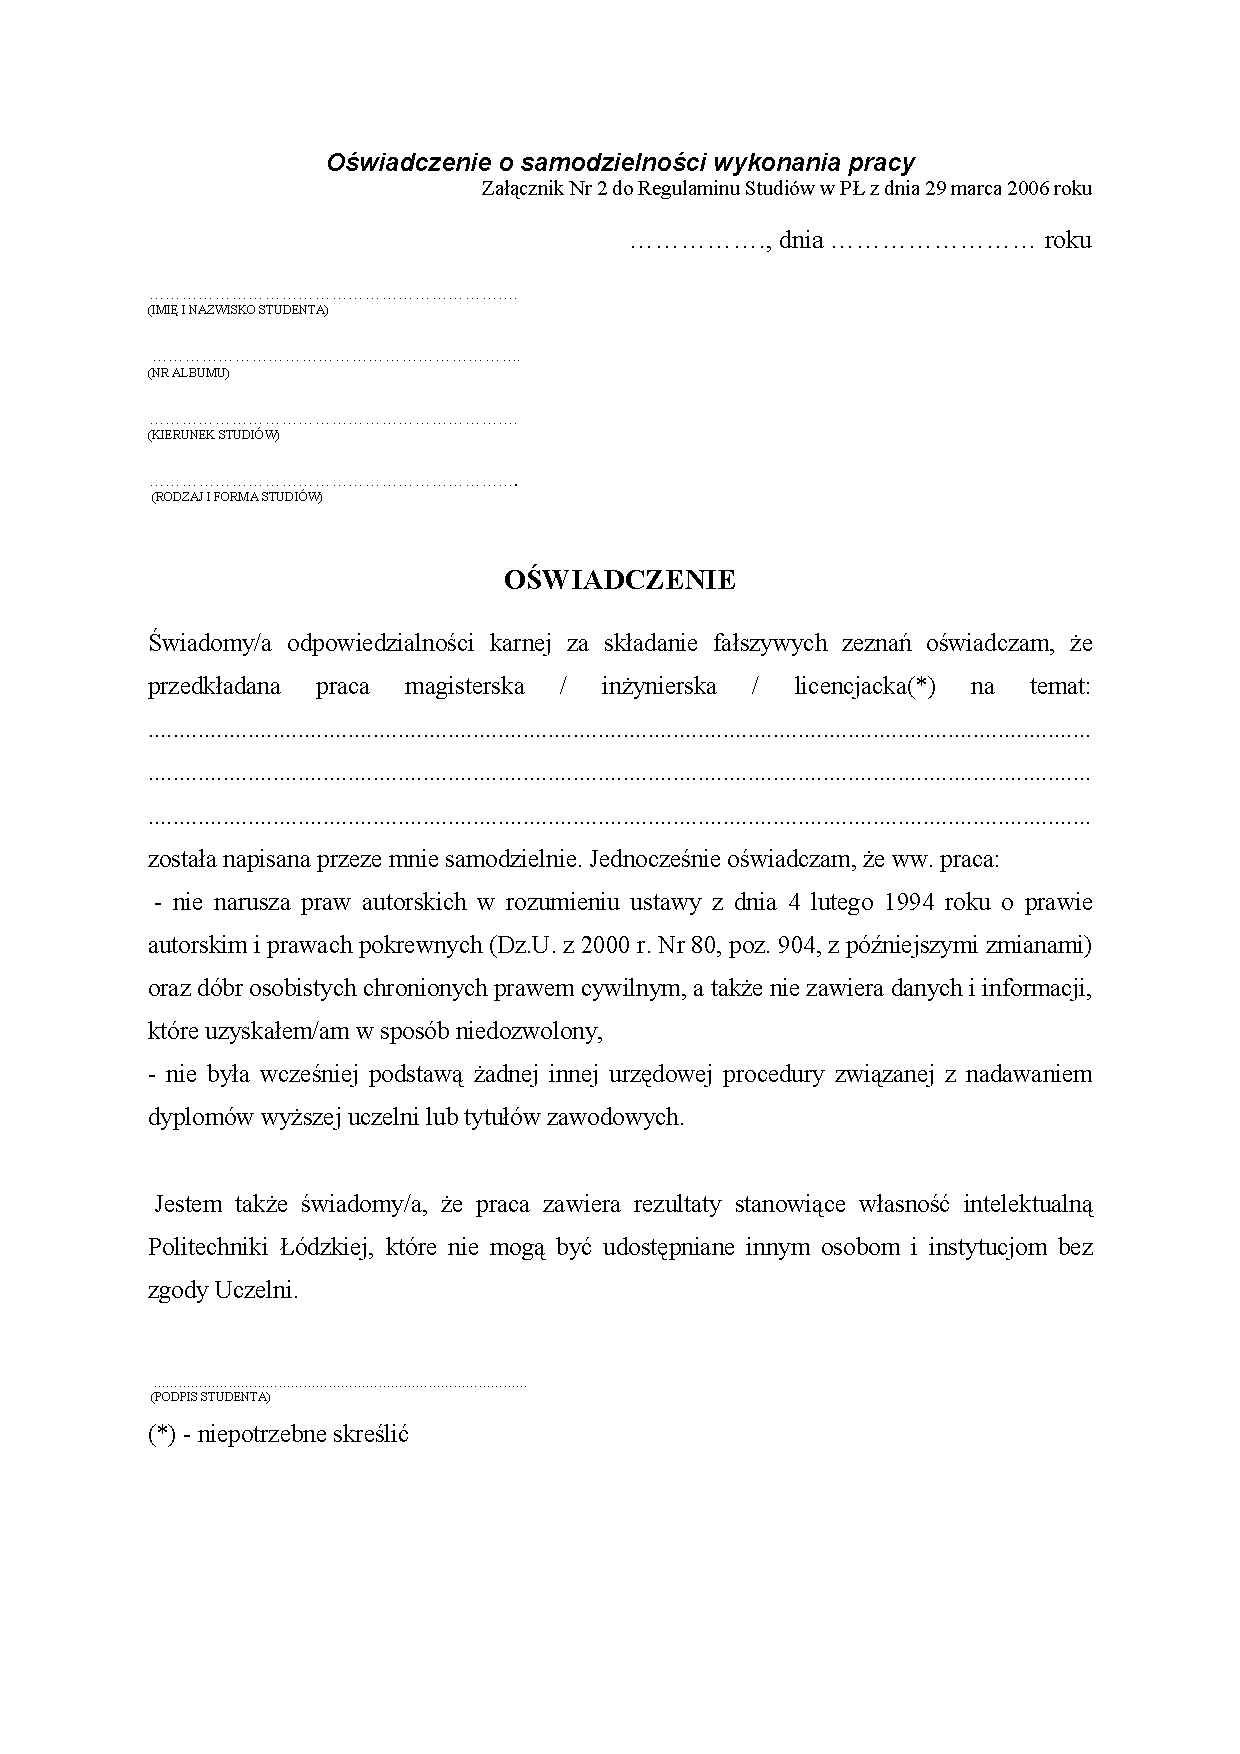
\includepdf[pagecommand={\thispagestyle{empty}}]{FrontBackmatter/declaration.pdf}
% ********************************************************************
% Game Over: Restore, Restart, or Quit?
%*******************************************************
\end{document}
% ********************************************************************
